\documentclass{PHlab-thesis}
\usepackage{amsmath}
\usepackage{amsfonts} 
\usepackage{graphicx}
\usepackage{algpseudocode}
\usepackage{algorithm}
\usepackage{float}
\usepackage{booktabs}
\usepackage[flushleft]{threeparttable}
\usepackage{subcaption}
\usepackage{multirow}
\addbibresource{thesis.bib}

\newcommand*\Department中文{醫學資訊研究所}
\newcommand*\Department英文{Institute of Medical Informatics}

\newcommand*\ThesisTitle中文{可視化轉錄因子結合位點與甲基化資訊之實現}
\newcommand*\ThesisTitle英文{Computational  pipeline for visualizing  transcription factor binding site with methylation information }
%\newcommand*\ThesisNote中文{示例:其實徐翡曼是東京大學畢業的博士}% For real thesis omit, or use {初稿} etc.
%\newcommand*\ThesisNote英文{Just an example.  Fei-Man actually graduated from Tokyo Univ.}% For real thesis omit, or use {draft} etc.

\newcommand*\Student中文{郭昱伶}
\newcommand*\Student英文{Yu-Ling Guo}

\newcommand*\Advisor中文{賀保羅}
\newcommand*\Advisor英文{Paul Horton}

%% 果有共同指導老師可以用:
%% \newcommand*\CoAdvisorA中文{}
%% \newcommand*\CoAdvisorA英文{}
%% \newcommand*\CoAdvisorB中文{}
%% \newcommand*\CoAdvisorB英文{}

\newcommand*\YearMonth英文{July, 2023}
\newcommand*\YearMonth中文{112年7月}

\hyphenpenalty=1024

\pagestyle{fancy}
\hyphenation{MethylSeq-Logos}
\hyphenation{MethylSeq-Logo}
\hyphenation{seq-uence}
\hyphenation{seq-uences}
\hyphenation{control-ling}
\hyphenation{methyl-ation}
\hyphenation{Th-ese}

\begin{document}


\newcommand*\Keywords英文{MethylSeqLogo, Transcription Factor, DNA methylation}
\newcommand*\Abstract英文{
%Background
Both transcription factor (TF) binding and DNA Methylation on or near genes are known to play important roles in gene regulation. Recently Hsu \& Horton developed MethylSeqLogo, as a "methylation smart" extension to sequence logos which simultaneously show the DNA sequence and methylation patterns of a collection of TF binding sites (vis-à-vis some background distribution).

Their MethylSeqLogo design appears useful to but their work has two limitations. The first limitation is that they did not fully automate the process of producing MethylSeqLogo images from primary data. This is problematic because both TF binding and DNA methylation are tissue specific, so every user potentially is interested in seeing a different MethylSeqLogo image. Hsu \& Horton do provide open source software to produce MethylSeqLogo images, but require the user to provide the information TF binding site sequence and methylation information shown in the images. Unfortunately, several steps are needed to extract that information from the standard primary or secondary data files widely available from the relevant experiments (CHiP Seq for TF binding and BiSulfite sequencing for DNA methylation).  The second limitation is they provide only two background distributions (whole genome and a set of promoter regions) against which to compared the DNA methylation level of TF binding sites, but the binding site distribution of some TFs may not fit either of those background models well.

%GOAL and Method
This work describes our development of original software to support and extend MethylSeqLogo. We 1) create an automated pipeline to automate the production of MethylSeqLogo's from experimental data in standard data file formats, and 2) extend the MethylSeqLogo software to support TF specific background models based on the regions flanking their binding sites.

%Results and discussion
After describing our implementation we show several MethylSeqLogo images generated using our pipeline. We confirm that those MethylSeqLogo images are consistent with the images published by Hsu \& Horton when using the same (whole genome) background model.  Furthermore we contrast the MethylSeqLogo images produced with a flanking region background model versus their promoter region background.  We find that in some cases for which the promoter background model seems to indicate an important role for DNA methylation, much of the apparent correlation between DNA methylation and binding disappears when using the flanking region background model.  This observation underscores the need for using a suitable background when interpreting statistical trends in data.}



\newcommand*\Keywords中文{甲基化序列標誌、轉錄因子、DNA 甲基化}
\newcommand*\Abstract中文{
%	背景:
	轉錄因子(TF)結合和基因附近的DNA甲基化在基因調控中扮演重要角色。Hsu和Horton在近期開發了MethylSeqLogo,作為序列標誌的「甲基化智能」擴展,它可以同時顯示一組轉錄因子結合位點的DNA序列和甲基化訊息(相對於某種背景分佈)。然而,他們的MethylSeqLogo設計有兩個限制。第一個限制是他們沒有完全自動化從原始數據生成MethylSeqLogo圖像的過程。這是一個大問題,因為TF結合和DNA甲基化是組織特異性的,所以每個使用者可能對不同的MethylSeqLogo圖像感興趣。Hsu和Horton提供了開源軟體來生成MethylSeqLogo圖像,但要求使用者提供在圖像中顯示的轉錄因子結合位點序列和甲基化訊息。不幸的是,從相關實驗的標準原始或次要數據文件中提取這些訊息需要幾個步驟(轉錄因子結合位的CHiP Seq和DNA甲基化的亞硫酸测序)。第二個限制是他們只提供了兩個背景分佈(whole genome 和 一組 promoter regions)來比較轉錄因子結合位點的DNA甲基化水平,但某些TF的結合位點分佈可能與這兩個背景模型都不匹配。
	
%	目標和方法:
	本研究描述了我們開發的原始軟體,以支持和擴展MethylSeqLogo。我們的目標是:1)創建一個自動化的計算管道,從標準數據文件格式(BED file)中自動生成MethylSeqLogo圖像的實驗數據;2)擴展MethylSeqLogo軟體,支持基於與TF結合位點側翼區域的TF特定背景模型flanking region)。
	
%	結果和討論:
	在描述我們的方法的實做之後,我們展示了使用我們的管道生成的幾個MethylSeqLogo圖像。當使用相同的(全基因組)背景模型時,我們確認這些MethylSeqLogo圖像與Hsu和Horton發佈的圖像一致。此外,我們對比了使用與啟動子區域背景(promoter region)相比的側翼區域(flanking region)背景模型生成的MethylSeqLogo圖像。我們發現在某些情況下,使用啟動子背景模型(promoter region)似乎表明DNA甲基化起著重要作用,當使用側翼區域背景模型(flanking region)時,DNA甲基化與結合位之間的大部分相關性消失。這個觀察強調了在解釋數據中的統計趨勢時使用適當背景的必要性。
}

\newcommand*\Acknowledgements{首先,我由衷感謝我的指導教授賀保羅老師。感謝您對我的指導和鼓勵,您專業知識和寶貴建議在整個研究過程中給予了我巨大的幫助,也豐富了我在生物基因領域方面的知識,在研究討論的過程中,讓我能更快速的找到研究問題解決的方向,再來也非常感謝劉宗霖老師與許釗凱老師,兩位口委老師給了我很多論文上的建議與教誨,使我的研究更加豐富且有深度。本研究的完成同時還要感謝 MethylSeqLogo 的主要作者之一 Fei-Man Hsu,與我分享研究時的寶貴經驗。

接者我要感謝實驗室的所有夥伴,學長姐-威穎、芊瑀、力元、宥霖以及恆霖;同屆夥伴-筱萱、怡靜、海墨、中柏、育丞以及益宗;學弟妹-映慈、其亮以及育晨,我們彼此教學相長,感謝你們提供課業及研究上的寶貴討論與協助,有你們的陪伴為我的研究所生活增添許多歡笑與色彩。

最後,我要感謝我最摯愛的爸爸、媽媽以及家人朋友們,感謝他們在我研究生涯的每一個階段給予我的無私支持和理解,你們的鼓勵和愛是我不斷前進的力量。再次感謝每一位給予我協助與鼓勵的人,您們的支持和幫助是我順利完成這項研究的關鍵。我將永遠珍惜這段寶貴的經歷。
\begin{flushleft}
謹向您們致以最誠摯的謝意,祝福您們身體健康、萬事如意。
\end{flushleft}

\begin{flushleft}
此致 \\
郭昱伶	
\end{flushleft}


}

\newcommand*\SelectFontsize[2]{\fontsize{#1}{#1}\selectfont\mdseries#2\par}
\newcommand*\SelectFontsizeBF[2]{\fontsize{#1}{#1}\selectfont\bfseries#2\par}
\newcommand*\SignatureRule[1][6]{\rule{#1cm}{0.3mm}}
\newcommand*\AddToContents[1]{\newpage\phantomsection\addcontentsline{toc}{chapter}{#1}}

\doublespace
\pagenumbering{gobble}
\renewcommand{\thefootnote}{\fnsymbol{footnote}}


\begin{center}
\vspace{2cm}
\SelectFontsizeBF{24}{%
\University中文\Department中文\\
\學位 論文}

\vfill
\SelectFontsizeBF{24}{\ThesisTitle中文}
\ifdefined\ThesisNote中文
\SelectFontsize{22}{\textit{\ThesisNote中文}}
\fi

\vspace{5mm}
\SelectFontsizeBF{22}{\ThesisTitle英文}
\ifdefined\ThesisNote英文
\SelectFontsize{20}{\textit{\ThesisNote英文}}
\fi

\vfill

\begin{minipage}{\linewidth}
{\setlength\tabcolsep{0pt}
%
\begin{tabular}{ Wr{5em} Wl{6em} Wr{5em} wl{7em} }
研究生:   & ~~\Student中文  &      Student: & ~~\Student英文\\
指導老師: & ~~\Advisor中文  &      Advisor: & ~~\Advisor英文\\
\ifdefined\CoAdvisorA中文
共同指導: & ~~\CoAdvisorA中文 &   Co-Advisor: & ~~\CoAdvisorA英文\\
\fi
\ifdefined\CoAdvisorB中文
         & ~~\CoAdvisorB中文 &   Co-Advisor: & ~~\CoAdvisorB英文\\
\fi
\end{tabular}
}
\end{minipage}

\vfill
\SelectFontsize{18}{%
National Cheng Kung University,\\
Tainan, Taiwan, R.O.C.\\
Thesis for \ifdef\PhD{Doctor of Philosophy}{Master of Science} Degree\\
\YearMonth英文}

\vfill
\SelectFontsize{20}{中華民國\YearMonth中文}
\end{center}
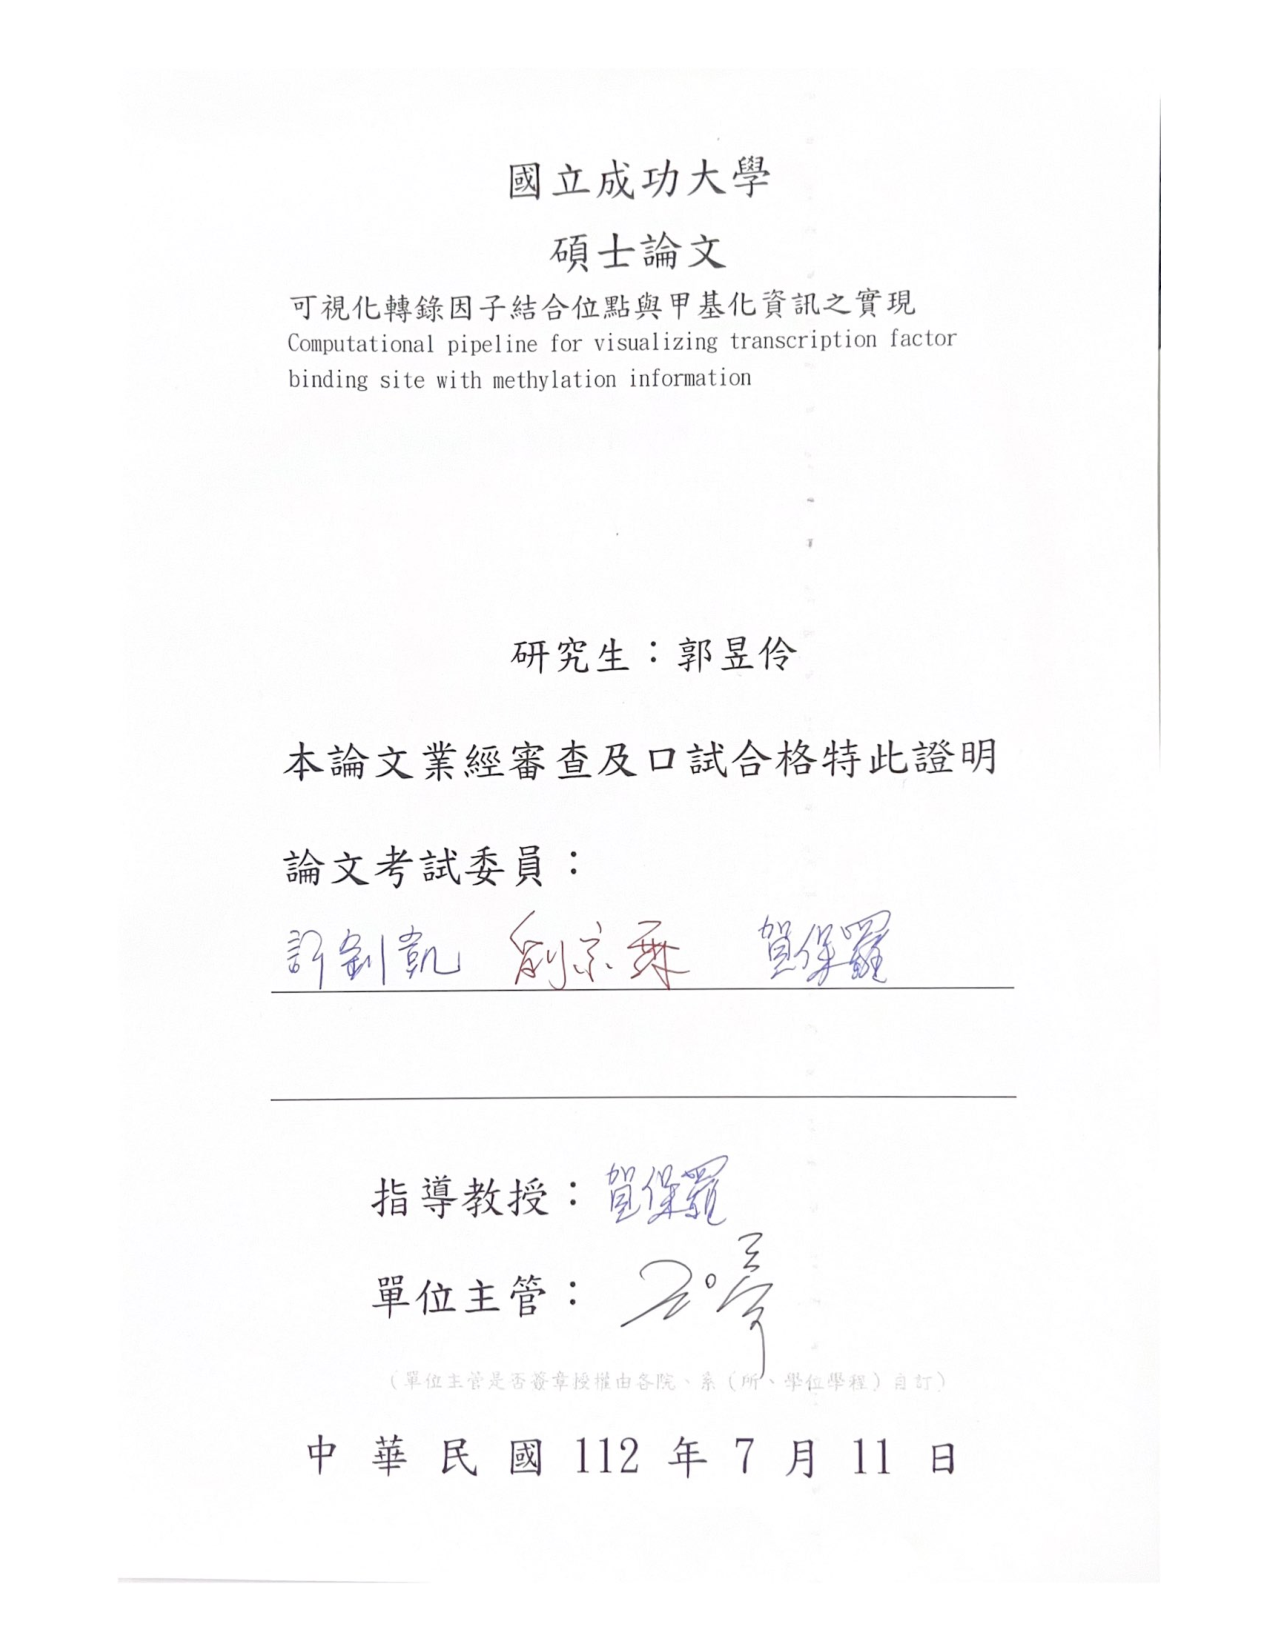
\includepdf[pages=1]{口試合格證明.pdf}


\ifdefined\optCommittee
\newpage
\begin{center}
\vspace{1cm}
\SelectFontsizeBF{24}{%
\University中文\Department中文\\
\學位 論文}
\vfill
\SelectFontsizeBF{20}{\ThesisTitle中文}
\end{center}

\vfill
\SelectFontsize{20}{%
\noindent 研究生:\Student中文\\
本論文業經審查及口試合格特此證明}


\begin{center}
\SelectFontsize{18pt}{論文考試委員}
\vfill
\SignatureRule \hspace*{1cm} \SignatureRule
\vfill

\SignatureRule \hspace*{1cm} \SignatureRule
\vfill

指導教授:\SignatureRule[8]
\vfill
  所長:\SignatureRule[8]

\vfill
\SelectFontsize{18}{中華民國 \hspace{2em} 年 \hspace{2em} 月 \hspace{2em} 日}
\end{center}


\newpage
\begin{center}
\vspace{1cm}
\SelectFontsize{18}{\University英文, \Department英文}
\SelectFontsize{19}{\ifdef\PhD{Ph.D.}{Master's} Degree Thesis}

\vfill
\SelectFontsizeBF{20}{\ThesisTitle英文}
\end{center}

\vfill
\SelectFontsize{18}{Student: \Student英文}

\SelectFontsize{18}{%
A thesis submitted to the graduate division in partial fulfillment of the requirement for the degree of
\ifdef\PhD{Doctor of \mbox{Philosophy}}{Master of Science}.
}

\vfill
\begin{center}
\SelectFontsize{18}{Approved by}

\vfill
\SignatureRule \hspace*{1cm} \SignatureRule

\vfill
\SignatureRule \hspace*{1cm} \SignatureRule

\vfill
Advisor: \SignatureRule[8]

\vfill
Chairman: \SignatureRule[8]

\vfill
\SelectFontsize{18}{\YearMonth英文}
\vspace*{20pt}
\end{center}
\fi% optCommittee


\AddToContents{中文摘要}
\setcounter{page}{1}
\pagenumbering{roman}


\begin{center}
\SelectFontsizeBF{24}{\ThesisTitle中文}

\vspace{4mm}
\SelectFontsize{18}{\Student中文\footnote[1]{學生} ~ \Advisor中文\footnote[2]{指導教授}}

\vspace{5mm}
\SelectFontsize{20}{國立成功大學\Department中文}

\vspace{12mm}
\makebox[2.7cm][c]{\SelectFontsizeBF{22}{摘要}}
\end{center}

\vspace{4mm}
\SelectFontsize{16}{\Abstract中文}

\vspace{4mm}
\begin{flushleft}
\SelectFontsize{16}{\textbf{關鍵詞:} \Keywords中文}
\end{flushleft}



\AddToContents{Abstract}
\begin{center}
\SelectFontsizeBF{22}{\ThesisTitle英文}

\vspace{4mm}
\SelectFontsize{18}{\Student英文\footnote[1]{Student} ~ \Advisor英文\footnote[2]{Advisor}}

\vspace{4mm}
\SelectFontsize{16}{\Department英文, National Cheng Kung University}

\vspace{12mm}
\SelectFontsizeBF{20}{Abstract}
\end{center}

\vspace{4mm}
\SelectFontsize{14}{\Abstract英文}

\vspace{4mm}
\begin{flushleft}
\SelectFontsize{16}{\textbf{Keywords:} \Keywords英文}
\end{flushleft}



\AddToContents{誌謝}
\begin{center}\SelectFontsizeBF{24}{誌謝}\end{center}

\vspace{4mm}
\Acknowledgements



\renewcommand{\contentsname}{CONTENTS}
\AddToContents{Contents}
\tableofcontents


\AddToContents{List of Tables}
\listoftables


\AddToContents{List of Figures}
\listoffigures
% 封面頁, 口委中英文簽名單, 誌謝, 中英文摘要, 論文目錄, 圖表目錄


%────────────────────  List of Symbols  ────────────────────
\renewcommand\nomgroup[1]{%
  \item[\bfseries
  \ifstrequal{#1}{A}{General}{%
  \ifstrequal{#1}{Z}{Gene/Protein Names}%
  }]}

% \nomenclature[A]{$\lg$}{Logarithm base 2}
% \nomenclature[A]{KL\ Divergence}{Kullback-Liebler Divergence}
% \nomenclature[Z]{Myc}{MYC proto-oncogene}
% \nomenclature[Z]{USF-1}{Upstream stimulatory factor 1}

\nomenclature[Z]{meC}{Methyl-Cytosine}
\nomenclature[Z]{TF}{Transcription Factor}
\nomenclature[Z]{bp}{Base Pair}
\nomenclature[Z]{DNA}{Deoxyribonucleic Acid}
\nomenclature[Z]{TFBS}{Transcription Factor Binding Site}
\nomenclature[Z]{H1-hESC}{Human Embryonic Stem Cells}

\nomenclature[A]{bg}{Background}


\printnomenclature[5cm]

\newpage
\setcounter{page}{1}
\pagenumbering{arabic}


\chapter{Introduction}
\section{Background}
During the process of biological growth, which includes cell growth, development, differentiation, apoptosis, and death, meticulous orchestration is required. It is akin to a production line where each step and pipeline of manufacturing and production influences the quality of the final product. Transcription factors (TFs) play a crucial role as key players in the growth of living organisms. TFs are proteins that regulate gene transcription, and upon interaction with DNA, they can control cellular logic by inhibiting or activating genes expression. This is why, despite all cells utilizing the same set of genes, there can be a wide variety of cell types (e.g., muscle cells, skin cells) with distinct functions. This diversity arises because only specific gene can be recognized and transcribed by TFs in different organs and tissues~\cite{lambert2018human}.

DNA methylation refers to the addition of a mn atom of cytosine, resulting in the formation of methyl cytosine (meC). It is often classified as the fifth DNA base~\cite{Listerfifthbase2009, Vinermethylsensitive2016} and is known to cause gene silencing and the abnormal functioning of genes, leading to inhibitory effects~\cite{Jones2012DNAmethylationislands}. DNA methylation is an epigenetic modification that can alter cellular gene function without changing the DNA sequence. Its effects can be inherited by the next generation. Numerous studies have shown a strong association between DNA methylation and cancer~\cite{KeithDNAmethyl2005, Feinberg1983Hypomethylation}.

A dinucleotide sequence may be considered too short and lack biological interest. However, CpG dinucleotides are an exception. In most vertebrate genomes, CpG dinucleotides are generally rare, occurring at a frequency of approximately one-fifth~\cite{Saxonov2006}. This is because they are prone to methylation by DNA methyltransferases. However, the situation is different in promoter regions. In many promoter regions, there is often a high density of consecutive CpG dinucleotides, forming gene sequences known as CpG islands. CpG islands are characterized by a relatively low or nearly absent level of methylation compared to the rest of the genome. This implies that genes within these regions are typically active and capable of transcription~\cite{Deaton2011CpG}.

Given that transcription is a complex and crucial process, it is of great importance to enable researchers to analyze and compare data efficiently and clearly. One early successful method in the field of molecular biology was the invention of "sequence logos"~\cite{schneider1990sequence}. Sequence logos provide a visual representation of transcription factor binding site (TFBS) preferences, allowing researchers to understand the binding preferences of transcription factors. A sequence logo consists of a stack of letters at each position (e.g., {A, C, G, T} for DNA sequences), where the height of each letter stack is proportional to the information content of the corresponding nucleotide distribution at that position~\cite{schneider1990sequence}. The widespread application of this method has demonstrated its utility in summarizing and visualizing binding sites, facilitating comparisons, and communicating transcription factor binding preferences among researchers. Sequence logo methods have been expanded in various ways, such as increasing the resolution of compositional enrichment/depletion (e.g., Seq2logo~\cite{Seq2Logo10.1093/nar/gks469} and EDlogo~\cite{Dey2018sequencelogo}), displaying higher-order sequence motifs~\cite{10.1093/nar/gky497}, or demonstrating relationships between binding site positions~\cite{Siebert2016Bayesian}.

Sequence logos help biologists understand the sequence preferences of transcription factors, but they cannot explain the cell-type-specific selection of TFBS (transcription factor binding sites). Therefore, additional information that affects transcription, such as DNA methylation and CpG dinucleotides, is required to gain a more comprehensive understanding of TF (transcription factor) function and quantify gene regulation within cells. 

Here, we introduce MethylSeqLogo~\cite{Hsu2022.11.05.515271}, a software tool that displays sequence logos with DNA methylation and CpG depletion as epigenetic information. Unfortunately, the MethylSeqLogo design appears useful too but their work has two limitations. The first limitation is that they did not fully automate the process of producing MethylSeqLogo images from primary data. This is problematic because both TF binding and DNA methylation are tissue-specific, so every user potentially is interested in seeing a different MethylSeqLogo image. Therefore, based on this idea, this study aims to provide computational pipelines for MethylSeqLogo, enabling researchers to utilize it extensively.
\section{Motivation \& Research objective}
The binding of transcription factors to DNA is a crucial mechanism for controlling gene expression in cells. For instance, humans possess approximately 1600\textasciitilde1700 different transcription factors, and through dynamic interactions with DNA, these transcription factors enable precise regulation of cellular processes such as growth, development, and response to the environment. Therefore, visualizing the binding sites of transcription factors to quantify gene regulation within cells has consistently been an important and necessary topic in life science research~\cite{vaquerizas2009census}~\cite{liu2017transcriptional}.

In a nutshell, this study explores the development of an automated computational pipeline for MethylSeqLogo~\cite{Hsu2022.11.05.515271} using tools and methods such as BEDTools~\cite{10.1093/bioinformatics/btq033}, Pandas~\cite{mckinney2010data}, seaborn~\cite{Waskom2021}, and others. The motivation behind this work stems from the observation that MethylSeqLogo currently only provides a limited set of pre-processed example files and lacks the functionality to accept the researcher's experimental raw data to generate results (sequence logo).

In addition to providing an automated computational pipeline, we propose a novel background model called the "flanking region." The background model is utilized to assess statistical differences associated with a set of binding sites, indicating the amount of relative entropy~\cite{kullback1951information} we can extract from the logos that produced by software .MethylSeqLogo currently provides the "whole genome" and a set of predefined "promoter" regions as background models. However,this study further focuses on the establishment of background regions specific to individual transcription factor binding sites, thereby tailoring customized background models for each transcription factor. The approach involves considering a defined range (e.g., 100 bp) of regions surrounding each binding site. Ideally, this process is performed independently for each binding site, resulting in the inclusion of x binding sites near genomic positions x times in the background model statistics. This ensures that the statistical differences depicted in the MethylSeqLogo visualization primarily arise from the binding sites themselves or their adjacent bases, rather than being influenced by large-scale trends in methylation and/or CpG frequency across the whole genome.

Here, we 1) create an automated pipeline to automate the production of MethylSeqLogo from experimental data in standard data file formats, and 2) extend the MethylSeqLogo software to support TF-specific background models based on the regions flanking their binding sites. The objective is to facilitate efficient and comprehensive observation of gene regulation within cells, including the extent of methylation, thereby providing valuable insights for academic research, analysis, and scientific communication. Furthermore, this research has potential implications for disease prevention and treatment.
\chapter{Related Work}
In this chapter, we will first give an overview of MethylSeqLogo~\cite{Hsu2022.11.05.515271}, and then introduce pybedtools~\cite{10.1093/bioinformatics/btr539} and the data required for this study to visualize MethylSeqLogo of transcription factor binding sites and methylation information, which are supported and provided by various databases. The following subsections provide a detailed explanation.
\section{MethylSeqLogo}
MethylSeqLogo~\cite{Hsu2022.11.05.515271} is an innovative tool known as DNA methylation smart sequence logos. It was proposed by Hsu \& Horton in 2022 as a "methylation smart" extension to sequence logos which simultaneously show the DNA sequence and methylation patterns of a collection of TF binding sites (visàvis some background distribution), providing insights into transcription factor functionality and gene regulation in cellular contexts.

Building upon traditional sequence logos, MethylSeqLogo intuitively represents the sequence conservation and preferences at each position in the DNA sequence. However, it expands this representation by incorporating DNA methylation information and highlighting CpG dinucleotide depletion in additional tracks. This enables researchers to gain a comprehensive understanding of the interplay between DNA methylation, transcription factor functionality, and gene regulation.
A detailed description of MethylSeqLogo shown in Figure\ref{fig:F1}. The column height of each track in MethylSeqLogo is determined by calculating the relative entropy (unit:bits), which represents the statistical distribution difference between a set of binding site sequences and the background model. Relative entropy, also known as the Kullback-Leibler directed divergence~\cite{kullback1951information}, is equivalent to information content~\cite{Information1986} when a uniform distribution background is used. The formula from MethylSeqLogo shown in  equation \ref{eu_eqn}:
\begin{equation} \label{eu_eqn}
	\text{D}(M||B) \overset{\text{def}}{=} \text{ E }\left [ \text{lg}\left (\frac{P[s|\text{Motif model M}]}{P[s|\text{Background model B}]} \right) \right]
\end{equation}
Here, is an example illustrating how to calculate the relative entropy from methylation. Suppose we want to calculate the relative entropy of mCG in a set of transcription factor binding sites (TFBSs) at position 1 in the whole genome background (plus strand). First, we need to calculate the probability of CG methylation level at the first position in all binding sites (P($^{\text{m}}\text{C}$|CG)), and the same calculation applies to the background model (whole genome). Furthermore, it is necessary to incorporate the information content of un-methylation, as it completes the full event. Lastly, since there are multiple binding sites, we also need to calculate the probability of the expected occurrence of CG dimer in the first position across all binding sites (P(C|CG)). The complete calculation process is as follows:
\begin{multline*}
	\text{Entropy} = \text{P}_{1}(\text{C}|\text{CG})*(\text{P}_{1}(^{\text{m}}\text{C}|\text{CG})*\text{lg}(\text{P}_{1}(^{\text{m}}\text{C}|\text{CG})/\text{P}_{\text{bg}}(^{\text{m}}\text{C}|\text{CG})))+\\
((1-\text{P}_{1}(^{\text{m}}\text{C}|\text{CG}))*\text{lg}((1-\texttt{P}_{1}(^{\text{m}}\text{C}|\text{CG}))/(1-\text{P}_{\text{bg}}(^{\text{m}}\text{C}|\text{CG}))))
\end{multline*}

\begin{figure}[H]
	\centering
	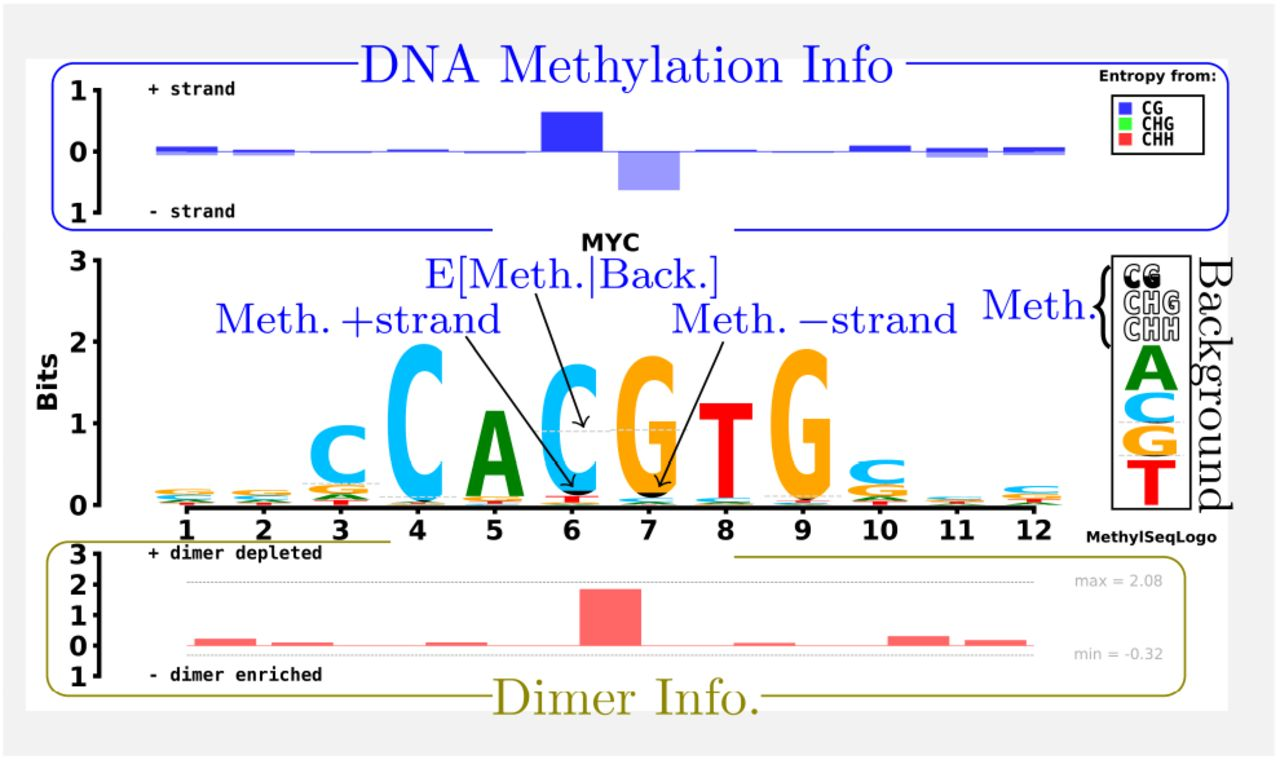
\includegraphics[scale=1]{figures/F1.large.jpg}
	\caption{Design of MethylSeqLogo (Figure is from~\cite{Hsu2022.11.05.515271},without changes)}
	\label{fig:F1} % \ref{this label}
\end{figure}

In summary, MethylSeqLogo provides a powerful and intuitive visualization tool for studying the functional role of DNA methylation in gene regulation. It is a valuable tool for researchers in the field of epigenetics and genomics, aiding in the identification of potential regulatory regions, examining the impact of DNA methylation on transcription factor binding, and gaining deeper insights into the complex gene regulatory processes occurring within cells.

\section{Pybedtools}
pybedtools~\cite{10.1093/bioinformatics/btr539} is a powerful Python library used for manipulating and analyzing genomic interval data. It serves as an interface to the BEDTools~\cite{10.1093/bioinformatics/btq033} suite, offering a wide range of functions to handle genomic intervals, including operations such as intersection, merging, and complementation between genomes. By leveraging the underlying BEDTools tools, pybedtools optimizes performance and memory usage, making it well-suited for efficient processing of large-scale genomic data. It supports various file formats, such as BED, BAM, VCF, and GTF, enabling easy reading and writing of data in different formats. Additionally, it provides advanced features like computing overlaps, calculating coverage statistics, and performing set operations. One significant advantage is its seamless integration with popular libraries like pandas and numpy, facilitating data analysis and calculations. Hence, pybedtools was chosen as a valuable tool for studying transcription factor binding sites in this research. Overall, pybedtools is a versatile and efficient tool for working with genomic interval data, offering an intuitive interface, extensive functionality, and integration with other Python libraries. The functions utilized in this study include "intersect" and "getfasta".
\begin{figure}[H]
	\centering
	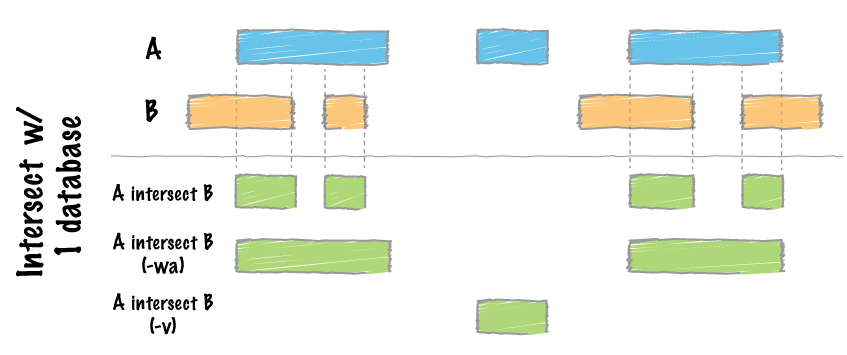
\includegraphics[scale=0.5]{figures/intersect-glyph.png}
	\caption{interesct method from BEDTools (Figure is from~\cite{10.1093/bioinformatics/btq033},without changes)}
	\label{fig:interesct} % \ref{this label}
\end{figure}
The figure shown in \ref*{fig:interesct} represent two BED files, labeled as A and B. In this study, BED file A represents the data obtained from JASPAR~\cite{10.1093/nar/gkab1113}, while BED file B corresponds to the data obtained from ReMap~\cite{ReMapFayrouz2022}.
\section{Database}
\subsection{JASPAR}
Transcription factor binding sites, also known as motifs, refer to specific DNA sequences where transcription factors bind and initiate transcription. Typically, the length of these sequences ranges from 5 to 20 nucleotides. JASPAR~\cite{10.1093/nar/gkab1113} is a freely accessible database that provides information on transcription factor binding sites. It serves as a valuable resource for conducting transcription factor - related analyses. JASPAR collects and analyzes transcription factor binding sites from six major species classifications, including fungi,insecta, nematoda, plantae, urochordata, and vertebrata. The database offers not only frequency matrices for transcription factor binding site locations but also provides additional data in the form of BED files, FASTA files, external links (such as ReMap and DRV), and more for researchers to download and utilize. In this study, we utilized the BED files from JASPAR, which provide the coordinates of transcription factor binding sites for each transcription factor across various cells or tissues. Furthermore, it is worth noting that in JASPAR the Matrix ID format typically follows the pattern of MAxxxx.x (e.g., MA0147.3), where the number after the decimal point represents the version of the datasets. A higher numerical value indicates a more recent version.

\begin{figure}[H]
	\centering
	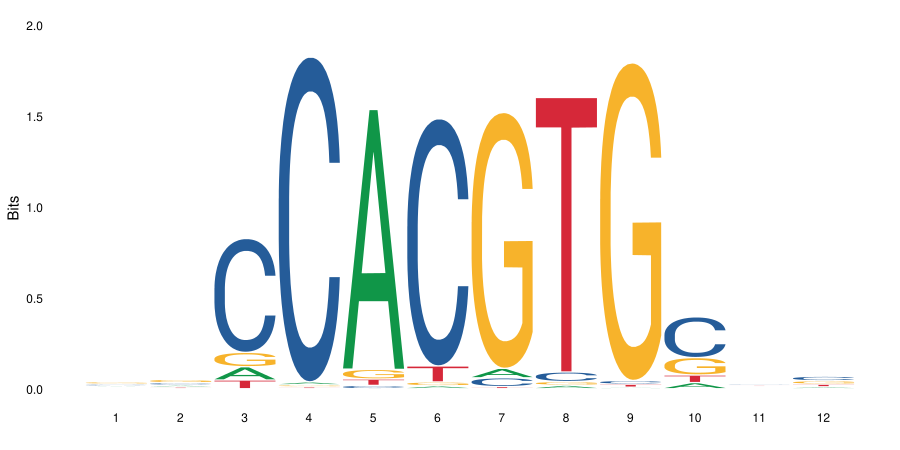
\includegraphics[scale=0.4]{figures/MA0147.3.png}
	\caption{Sequence logo of MYC (Figure is from~\cite{10.1093/nar/gkab1113},without changes)}
	\label{fig:MA0147} % \ref{this label}
\end{figure}

\subsection{ReMap}
If we are interested in identifying transcription factor binding sites in different cells or tissues, we can perform ChIP-seq experiments. ChIP-Seq is an experimental techinque which can measure the approximate positions of the binding sites of a given transcription factor to within 100–250bp. The identification of the most probably site within that range is done computationally based on the known binding sequence preferences of the transcription factor. In these experiments, we obtain numerous peaks, with each peak representing a potential transcription factor binding site within a specific region. Fortunately, ReMap~\cite{ReMapFayrouz2022} has organized this information for us. ReMap is a large-scale database of transcriptional regulatory peaks, which collects and analyzes data from ChIP-seq, ChIP-exo, and DAP-seq experiments. It covers various species, including humans, mice, fruit flies, and Arabidopsis, and provides analysis for a total of 1210 transcription factors. ReMap offers the data in both BED file and FASTA file formats, allowing users to download experiment-related information. For this study, we utilized the BED files containing ChIP-seq data from ReMap.

\begin{figure}[H]
	\centering
	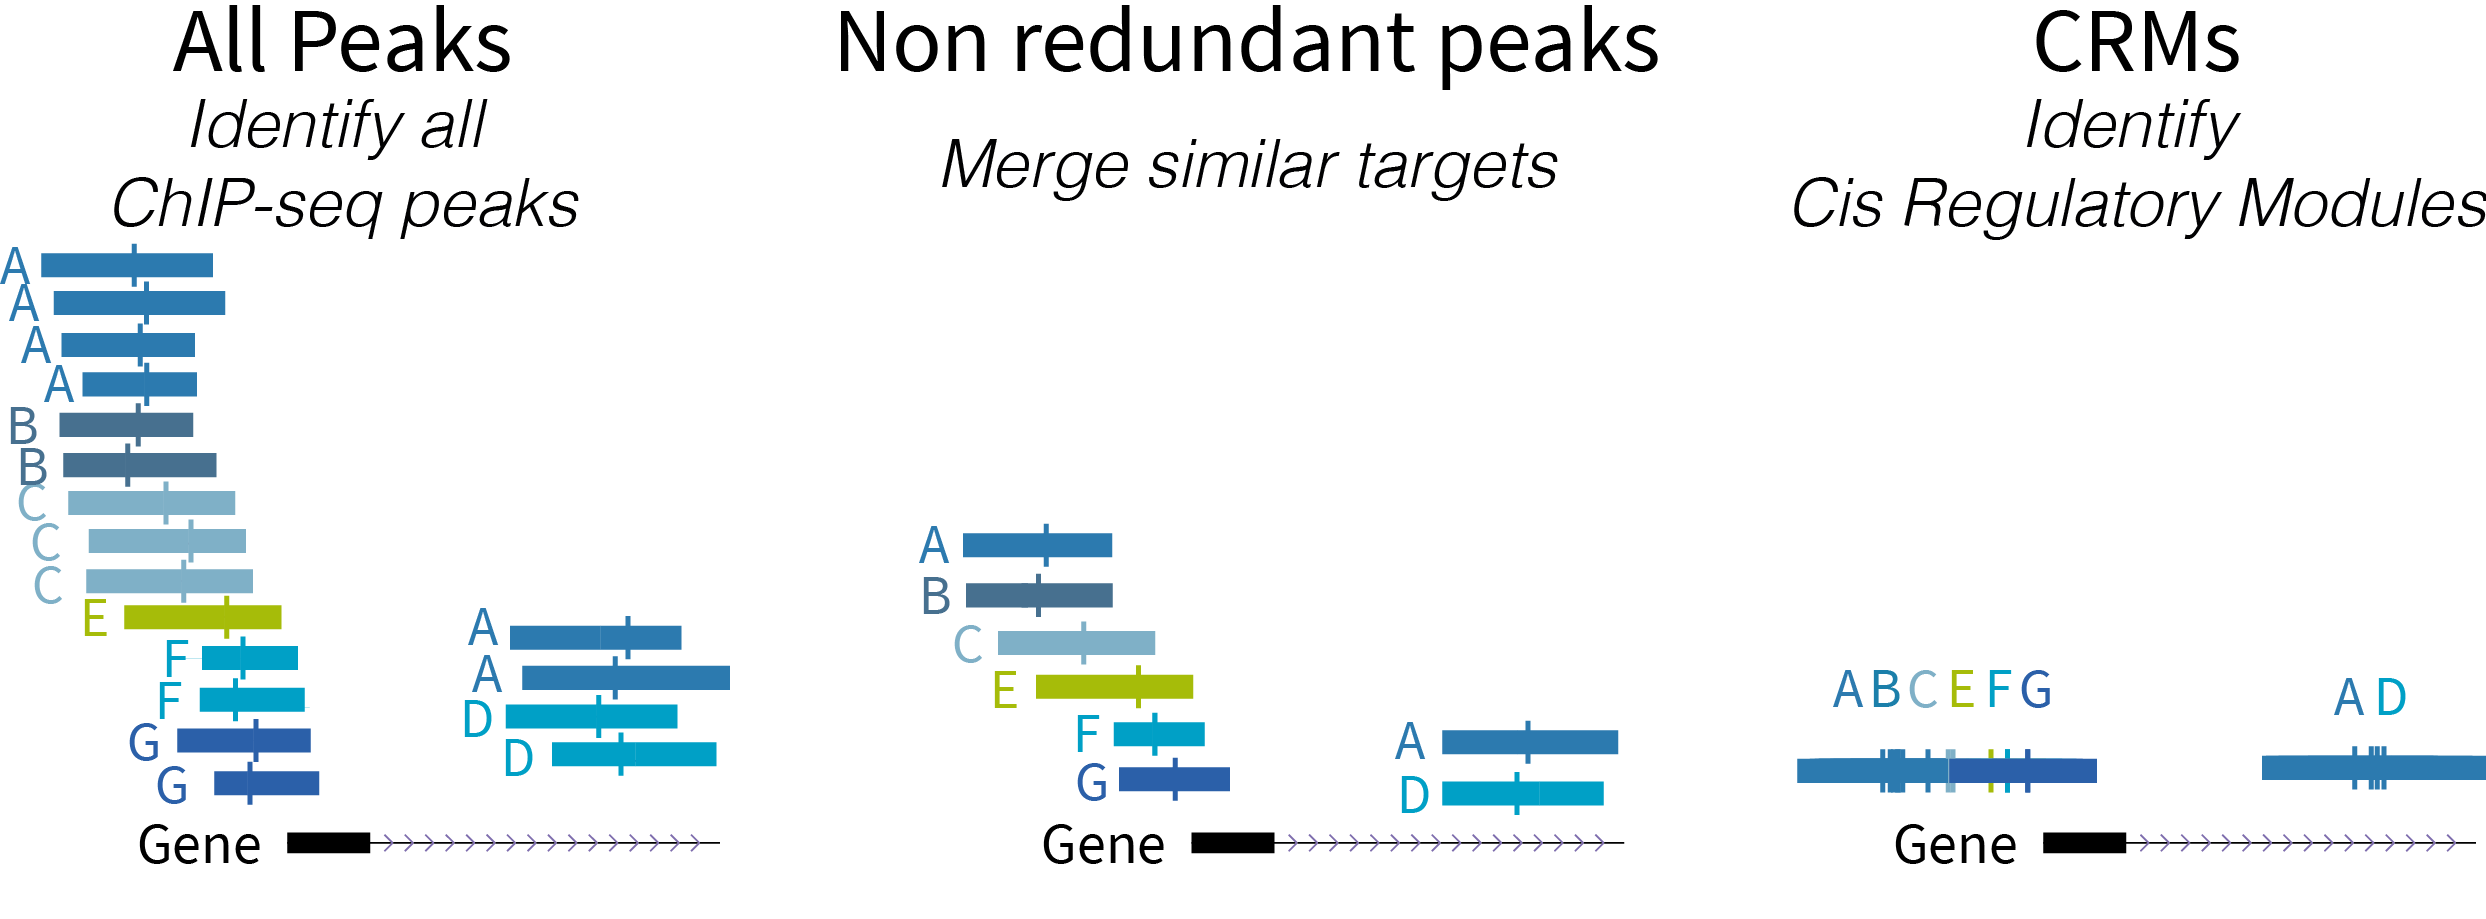
\includegraphics[scale=0.5]{figures/schema_data_remap2020_2.png}
	\caption{Schema data of ReMap (Figure is from~\cite{ReMapFayrouz2022},without changes)}
	\label{fig:remap} % \ref{this label}
\end{figure}

\subsection{ENCODE}
ENCODE~\cite{encode2012integrated} (Encyclopedia of DNA Elements) is a research project initiated by the National Human Genome Research Institute (NHGRI) in the United States in 2003. Its aim is to establish a comprehensive catalog of functional elements on the human genome, including DNA hypersensitive sites, DNA methylation, and transcriptional regulatory regions, among other experimental aspects. ENCODE researchers employ various assays and methods to identify functional elements, and all generated data is made available for download through their website for user analysis. In this study, DNA methylation data from ENCODE was utilized. Through sodium bisulfite sequencing, the binding of bisulfite to Cytosine (C) bases can be examined, leading to deamination. After the experimental process, unmethylated Cytosine bases are converted to Uracil (U) bases, while methylated Cytosine bases remain as Cytosine. This enables the acquisition of methylation information from the sequence, which is recorded in BED file format,but is distinct from JASPAR and ReMap, not only includes the basic sequence coordinate information but also records the read count and methylation level, thus referred to as bedMethyl, and shown in Table \ref*{table:bedMethyl}.
\begin{table}[H]
	\centering
	\begin{tabular}{l*{5}{c}}
		chromosome         & start coordinates &  end coordinates&...  & read coverage & methylation level(\%)\\
		\hline
		chr1 & 869 & 870 & ... & 8 & 50  \\
		chr1  & 1450 & 1451 & ... & 2 & 0  \\
		chr2   & 520 & 521 & ... & 4 & 38  \\
		chr2   & 14755 & 14756 & ... & 5 & 90  \\
		chr3   & 15449 & 15450 & ... & 8 & 0  \\
		\hline
	\end{tabular}
	\caption{Example of bedMethyl file from ENCODE}
	\label{table:bedMethyl}
\end{table}

\begin{figure}[H]
	\centering
	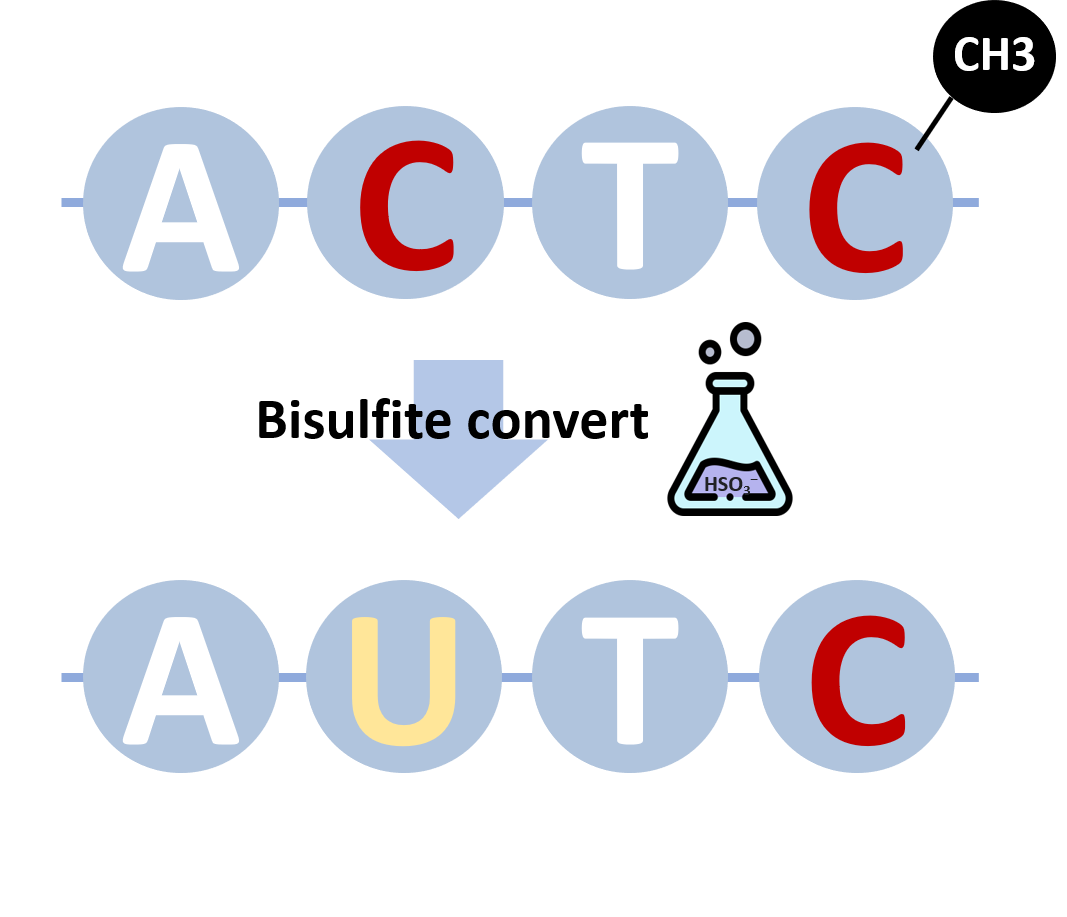
\includegraphics[scale=0.65]{figures/wgbs.png}
	\caption{The principle of WGBS}
	\label{fig:wgbs} % \ref{this label}
\end{figure}

\chapter{Methods}
In this chapter, the framework and workflow of my research methodology will be presented and discussed.
\section{Data flow of automatic computational pipeline for MethylSeqLogo}
Pipeline overview for MethylSeqLogo as shown in \ref{fig:overview}, the user is required to input files obtained from various experiments or databases. Files from ReMap and JASPAR contain relevant information about transcription factors and their binding sites, while files from ENCODE contain information about cellular methylation levels. Next, we will search for all binding site information of transcription factors in the cells and define our background model. We then calculate the methylation levels and the probabilities of base occurrence for each of the three methylation scenarios. Subsequently, we employ Relative Entropy to assess the statistical differences between the binding site distribution and the background model. Finally, we visualize the entropy on a image as the final output. In the following subsection, I will provide a more detailed and concrete explanation of the research methodology using the example of observing the gene regulation of the transcription factor MYC in human embryonic stem cells (H1-hESC).

\begin{figure}[H]
	\centering
	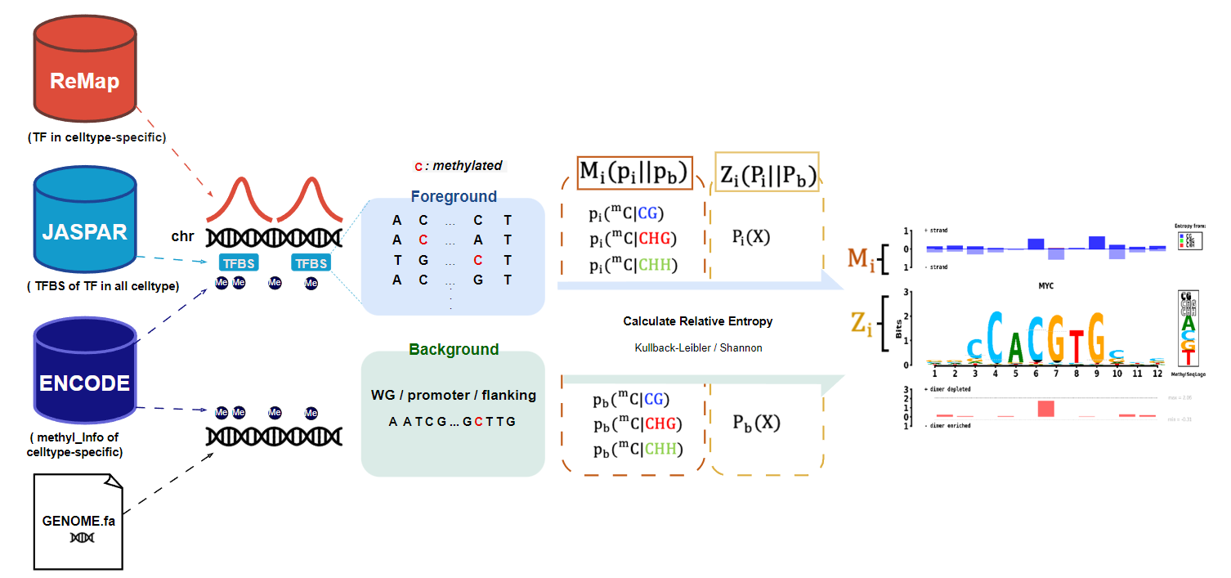
\includegraphics[scale=0.5]{figures/OVERVIEW.png}
	\caption{Pipeline overview}
	\label{fig:overview} % \ref{this label}
\end{figure}

\section[Automatic Computational Workflow]{Detail workflow of automatic computational pipeline}
\subsection[Finding TFBSs]{Identifying the binding site information of TF in cell.}
In this step, two input files are required. The first file contains the regions obtained from the Chip-seq experiment, which potentially contain the binding sites of MYC in human embryonic stem cells. These regions are represented as approximate genomic coordinates and typically have a range of 200-500 base pairs. This data can be obtained from ReMap, and the specific file I used is "ENCSR000EBY.MYC.WA01.bed". The second file can be obtained from JASPAR and contains the precise binding site coordinates of the MYC transcription factor across various cells or tissues. The file I used is "MA0147.3.bed". Both files obtained from ReMap and JASPAR are in the BED file format. We can then intersect the genomic coordinates from these two files to find the binding site information of MYC in human embryonic stem cells (H1-hESC). In the automated computational pipeline, this study used the "intersect" function provided by the pybedtools library in BEDTools to perform this operation. A total of 2088 transcription factor binding sites of MYC were found.
It is important to note that both files must be mapped to the same human reference genome. Genomic coordinates generated based on different human reference genomes can vary significantly. The commonly used human reference genomes are hg19 and hg38, with hg38 being more prevalent. This is because hg38 has improved genome coverage compared to hg19, resulting in more accurate positioning and annotation of gene sequences. Furthermore, some structural errors in chromosomes have been corrected in hg38. Fortunately, we can quickly convert the genomic coordinates between hg19 and hg38 using the "Lift Genome Annotations" website provided by UCSC.
\begin{figure}[H]
	\centering
	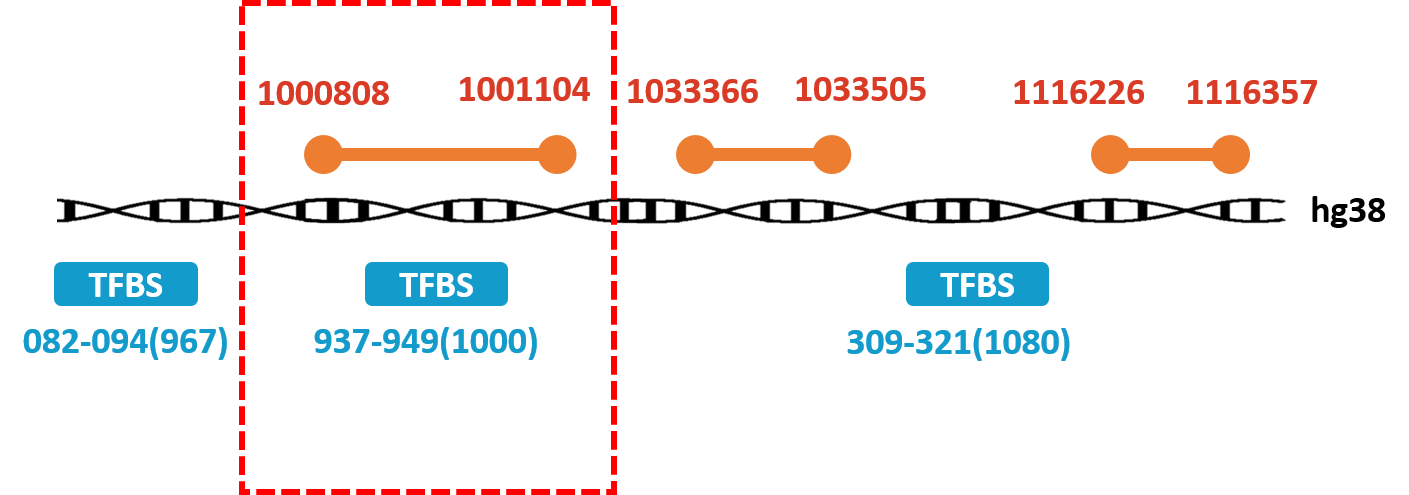
\includegraphics[scale=0.6]{figures/findTFBSs.png}
	\caption{Illustration of Finding Transcription Factor Binding Sites in Cell }
	\label{fig:findTFBSs} % \ref{this label}
\end{figure}
In \ref{fig:findTFBSs}, the orange and blue colors represent data from ReMap and JASPAR, respectively. The numbers indicate the coordinates of the gene sequence. The interpretation of "082-094 (967)" is that the gene sequence spans from coordinate 967082 to coordinate 967097. From the figure, we can see that the red dashed box represents the intersection, indicating that the gene fragment from coordinate 1000937 to 1000949 is the binding site of MYC in human embryonic stem cells (H1-hESC).

\subsection{Data preprocessing} \label{sssec:num1}
Once the binding sites are identified, we need to convert the coordinate data into sequence data. In our automated computational pipeline, we also utilize pybedtools to accomplish this task. The specific command used is "tfbs. sequence (fi=fasta)". In this command, "tfbs" refers to the BED file containing the binding sites of MYC in human embryonic cells that we just found, and "fasta" refers to the human reference genome file (version: hg38), it's a FASTA format file, which can be downloaded from the Illumina iGenomes website.
\begin{table}[H]
	\centering
	\begin{tabular}{l*{12}{c}}
		\toprule
		         & 1 &  2&  3&4  &5&6&7&8&  9& 10 & 11&12\\
		\midrule
		chr1:1000935-1000951(+)     & C  &G  &C  &C  &A  &C  &G  &T  &G  &C  &T  &T		\\
		chr1:1232506-1232522(-)      &A  &G  &C  &C  &A  &C  &G  &T  &G  &C  &T  &G\\
		...   &.. &.. &.. &.. &.. &.. &.. &.. &.. &.. &.. &..\\
		
		chrX:154763520-154763536(-)  &C  &A  &C & C & A  &C  &G  &T  &G  &G  &C  &T\\
		chrX:154763547-154763563(+) & C  &G  &A  &C  &A  &C  &G  &T  &G  &C  &A  &G\\
		\bottomrule
	\end{tabular}
	\caption{Example of dataframe with seqdata}
	\label{table:seqdata}
\end{table}
Once we obtain the sequence data, we can calculate the probability of occurrence for each \{ A, C, G, T \} nucleotide at each position within a set of binding sites using the ppm calculation. By comparing this probability distribution to the background statistical distribution and calculating the Relative Entropy, we can generate the sequence logo, which represents the transcription factor's binding site preference information displayed in the central track. It is worth mentioning that in our automated computational pipeline, we use the sequence data to construct a dataframe that records the methylation condition for the C/G base, shown in ~\ref{table:ctx}. This dataframe is used for the convenient calculation of methylation levels in subsequent analyses.
\begin{table}[H]
	\centering
	\begin{tabular}{l*{12}{c}}
		\toprule
		         & 1 &  2&  3&4  &5&6&7&8&  9& 10 & 11&12\\
		\midrule
	
		0     &X  &x  &Z  &Z  &-  &X  &x & -  &z  &Z  &-  &-\\
		1     &-  &X  &x  &y  &-  &X  &x  &-  &X  &x  &-  &X\\
		...   &.. &.. &.. &.. &.. &.. &.. &.. &.. &.. &.. &..\\
		2062  &z  &z  &z  &z  &-  &z  &Z  &- &Y   &X &x  &z\\
		2088  &X  &x  &-  &Z  &-  &X  &x  &-  &z  &Y  &-  &y\\
		\bottomrule

	\end{tabular}
	\begin{minipage}{9.5cm}
		\vspace{0.15cm}
		\footnotesize  Notes: X: CG, Y: CHG, Z: CHH (Uppercase and lowercase letters represent the plus and minus strands, respectively)
		\end{minipage}
	\caption{Example of dataframe with methylation condition}
	\label{table:ctx}
\end{table}

Regarding the methylation of TFBSs, the combination of \{CG, CHG, CHH\} is sufficient to describe the DNA methylation condition. Here, H represents any nucleotide except for G in the plus strand. However, during the WGBS experiment, some experimental errors or biases may occur.  We downloaded WGBS data from the ENCODE website for the H1-hESC cell line. The ENCODE IDs for the downloaded data are ENCFF601NBW, ENCFF918PML, ENCFF524BMX, ENCFF379ZXG, ENCFF086MMC, and ENCFF417VRB. These files represent methylation at CG, CHG, and CHH contexts, with two files for each context. To enhance the reliability of methylation level estimation.

To calculate the methylation of TFBSs, we utilized the intersect function in pybedtools to intersect the WGBS BED file with the BED file containing MYC binding sites in the H1-hESC cell line (generated in Section 3.2.1). The process is similar to the TFBS identification. After that, we can obtain the methylation levels of TFBSs.

Here, we will explain how the study handles the two replicates of WGBS files for each methylation context. The calculation formula used to merge two replicates files is shown in ~\ref{merge}. In the automated computational pipeline, the study organizes the six WGBS files into two dataframe tables. These tables record the counts of methylated reads and unmethylated reads, respectively. Table 3.1 serves as the main table, while Tables 3.2 and 3.3 provide supplementary information. By referencing these tables, the methylation levels and probabilities of \{ CG, CHG, CHH \} at each position within a set of binding sites can be calculated using a table lookup approach. The relative positions of each dataframe are interconnected, enabling the calculation based on their respective locations.\begin{small}
\begin{equation} \label{merge}
	 \text{mlevel} = \frac{^{\text{methylated}}\text{reads}_{\text{A}} + ^{\text{methylated}}\text{reads}_{\text{B}}}{(^{\text{methylated}}\text{reads}_{\text{A}} + ^{\text{unmethylated}}\text{reads}_{\text{A}})+ (^{\text{methylated}}\text{reads}_{\text{B}} + ^{\text{unmethylated}}\text{reads}_{\text{B}})}
\end{equation}
\end{small}
\begin{table}[H]
	\centering
	\begin{tabular}{l*{12}{c}}
		\toprule
		         & 1 &  2&  3&4  &5&6&7&8&  9& 10 & 11&12\\
		\midrule
		
		0     &13.0  &10.0  &13.0  &13.0   &NaN  &13.0  &11.0   &NaN &11.0  &11.0   &NaN   &NaN\\
		1     &NaN   &0.0  &24.0  &14.0  &NaN  &13.0  &23.0   &NaN  &24.0  &24.0  &NaN   &0.0\\
		...   &.. &.. &.. &.. &.. &.. &.. &.. &.. &.. &.. &..\\
		
		2062   &0.0  &20.0  &30.0  &30.0   &NaN  &30.0  &28.0   &NaN  &28.0  &28.0   &0  &28.0\\
		2088 &22.0  &13.0   &NaN  &23.0   &NaN  &23.0  &13.0  &NaN  &13.0  &23.0   &NaN  &13.0\\
		\bottomrule
	\end{tabular}
	\begin{minipage}{15.5cm}
		\vspace{0.1cm}
		\footnotesize  Notes 1: The number represents sum of unmethylated read counts from two replicate WGBS files for each \{CG, CHG, CHH\} condition. (NaN:the base in that field is A/T (adenine/thymine))
	\end{minipage}
	\caption{Example of dataframe with unmethylation read counts record}
	\label{table:unmethylated}
\end{table}
\begin{table}[H]
	\centering
	\begin{tabular}{l*{12}{c}}
		\toprule
		         & 1 &  2&  3&4  &5&6&7&8&  9& 10 & 11&12\\
		\midrule
		
		0     &0.0  &0.0  &0.0  &0.0   &NaN  &0.0  &0.0   &NaN &0.0  &0.0   &NaN   &NaN\\
		1     &NaN   &0.0  &0.0  &0.0  &NaN  &0.0  &0.0   &NaN  &0.0 &0.0 &NaN   &0.0\\
		...   &.. &.. &.. &.. &.. &.. &.. &.. &.. &.. &.. &..\\
		
		2062   &0.0  &0.0  &0.0  &0.0  &NaN  &0.0  &0.0   &NaN  &0.0  &0.0   &0.0  &0.0\\
		2088 &1.0  &0.0   &NaN  &0.0   &NaN  &0.0  &0.0  &NaN  &0.0  &0.0   &NaN  &0.0\\
		\bottomrule
	\end{tabular}
	\begin{minipage}{14cm}
		\vspace{0.15cm}
		\footnotesize  Notes 1: The number represents sum of methylated read counts from two replicate WGBS files for each \{CG, CHG, CHH\} condition. (NaN:the base in that field is A/T (adenine/thymine)) 
	\end{minipage}
	\caption{Example of dataframe with methylation read counts record}
	\label{table:methylated}
\end{table}

\subsection{Calculate the methylation probability of the background model}
In the previous subsection, we discussed the methylation probabilities of binding sites. Therefore, here we will explain the calculation of methylation probabilities in the background model. For this, WGBS (whole genome bisulfite sequencing) data from the H1-hESC cell line are required, as described in subsubsection~\ref{sssec:num1}. The approach involves reading two WGBS files with the same methylation status, and they must be sorted. Since the failure rate of WGBS experiments is very low, the content of the files obtained from the same cells will have highly similar or even identical coordinates. The differences lie in the read coverage and methylation ratio, which may vary slightly due to experimental variations. Based on this idea, we can merge the methylation levels of the same coordinates in the two files (the pseudocode for the condition should include an OR statement). The same approach applies to different background models, with the only difference being the size of the data used. Various background models are filtered using the pybedtool intersect function.


\subsection{About Flanking region}
The new background model option presented in this study, called "flanking regions," is designed to tailor the background model specifically to a set of binding sites. The method involves extending the starting and ending genomic coordinates of a set of binding sites by a range, say 100 base pairs, on either side. The total length of the range is equal to twice the extended range length (since there are both left and right sides). This ensures that the statistical differences described in MethylSeqLogo can be attributed to the binding site or its neighboring flanking nucleotides, rather than large-scale trends. Large-scale trends can sometimes amplify effects and lead to confusion in the interpretation of the information we are interested in.
\subsection{The execution time and memory usage of the automated computational pipeline }
In the automated computational pipeline established in this study, in addition to addressing the lack of automation in the original MethylSeqLogo and providing a new background model option, we have also made improvements to address two additional issues. The first issue pertains to insufficient memory space. As shown in table~\ref{table:WGBSinfo}, the six WGBS files from ENCODE have a combined size of approximately 100GB for CHH methylation data. When calculating the methylation probabilities for the background model, it would require occupying 80\% of the memory, which is highly undesirable and could lead to program failure. To overcome this problem, I adopted a window-like concept, reading one line at a time from the files, instead of loading all files into memory at once to prevent memory space issues.
The second issue relates to the excessively long execution time due to the large file sizes, which is the second aspect of improvement. To address this problem, I employed the multiprocessing package to implement parallel computing, thereby accelerating the calculation of methylation probabilities.
	
\begin{table}[H]
	\centering
	\scalebox{0.65}{
	\begin{tabular}{l*{6}{c}}
		
				& Methyl-codition      & Celltype                 & File capacity(GB) & original~execution time(min)~ & after implementing parallel(min)  \\
		\hline
				ENCFF417VRB & \multirow{2}{*}{CHH} & \multirow{6}{*}{H1-hESC} & 50.92             & \multirow{2}{*}{144}          & \multirow{2}{*}{27}               \\
				ENCFF086MMC &                      &                          & 51.3              &                               &                                   \\
				ENCFF524BMX & \multirow{2}{*}{CHG} &                          & 14.69             & \multirow{2}{*}{44}           & \multirow{2}{*}{8}                \\
				ENCFF379ZXG &                      &                          & 14.57             &                               &                                   \\
				ENCFF601NBW & \multirow{2}{*}{CpG} &                          & 3.44              & \multirow{2}{*}{6}            & \multirow{2}{*}{2}                \\
				ENCFF918PML &                      &                          & 3.47              &                               &                                  
	
	\end{tabular}}
	\caption{Detailed information about the WGBS files from the ENCODE}
	\label{table:WGBSinfo}
\end{table}
In conclusion, this chapter has provided detailed explanations of the methods and procedures for finding binding sites, a serial of data preprocessing, various probability calculations (base frequency and methylation), and the workflow shown in ~\ref{fig:Automatipipeline}. It is important to note that since DNA is double-stranded, the methylation probability calculation should consider the information from both the forward and reverse strands. With the calculated probabilities, we can now proceed to calculate the relative entropy between a set of binding sites and the background model, enabling the generation of a MethylSeqLogos image. The calculation method and graphical presentation of relative entropy follow the specifications and design of the original MethylSeqLogo.
\clearpage
\begin{figure}
	\centering
	\includegraphics[scale=0.1]{figures/0710.png}
	\caption{Workflow of automatic computational pipeline}
	\label{fig:Automatipipeline} 
\end{figure}

\chapter{Results} 
In this chapter, we will discuss whether the content mentioned in the literature or reports regarding transcription factors aligns with the visual presentation of our study's sequence logo. Tests were executed on a Linux server with a single AMD RyzenTM 9 5950X desktop processor, consisting of 16 hyper-threaded physical cores running at their base clock 3.4GHz, and 128GB of random access memory.
\section{MYC in H1-hESC cell line}
The transcription factor MYC belongs to the helix-loop-helix family and possesses characteristic structural features of a basic region and a leucine zipper. It is an important transcription factor that plays a crucial role in processes such as cell growth, metabolism, angiogenesis, and immune response. It is considered a significant oncogene, as its overexpression has been associated with abnormal cell proliferation in many tumors. According to the research conducted by Michael Allevato et al., the preferred sequence for the binding site of the MYC transcription factor is CANNTG, with the CACGTG sequence being the most highly favored and preferred~\cite{allevato2017sequence}. The visualization in~\ref{fig:MYC} demonstrates consistency with the reported findings.
\begin{figure}[H]
	\centering	
	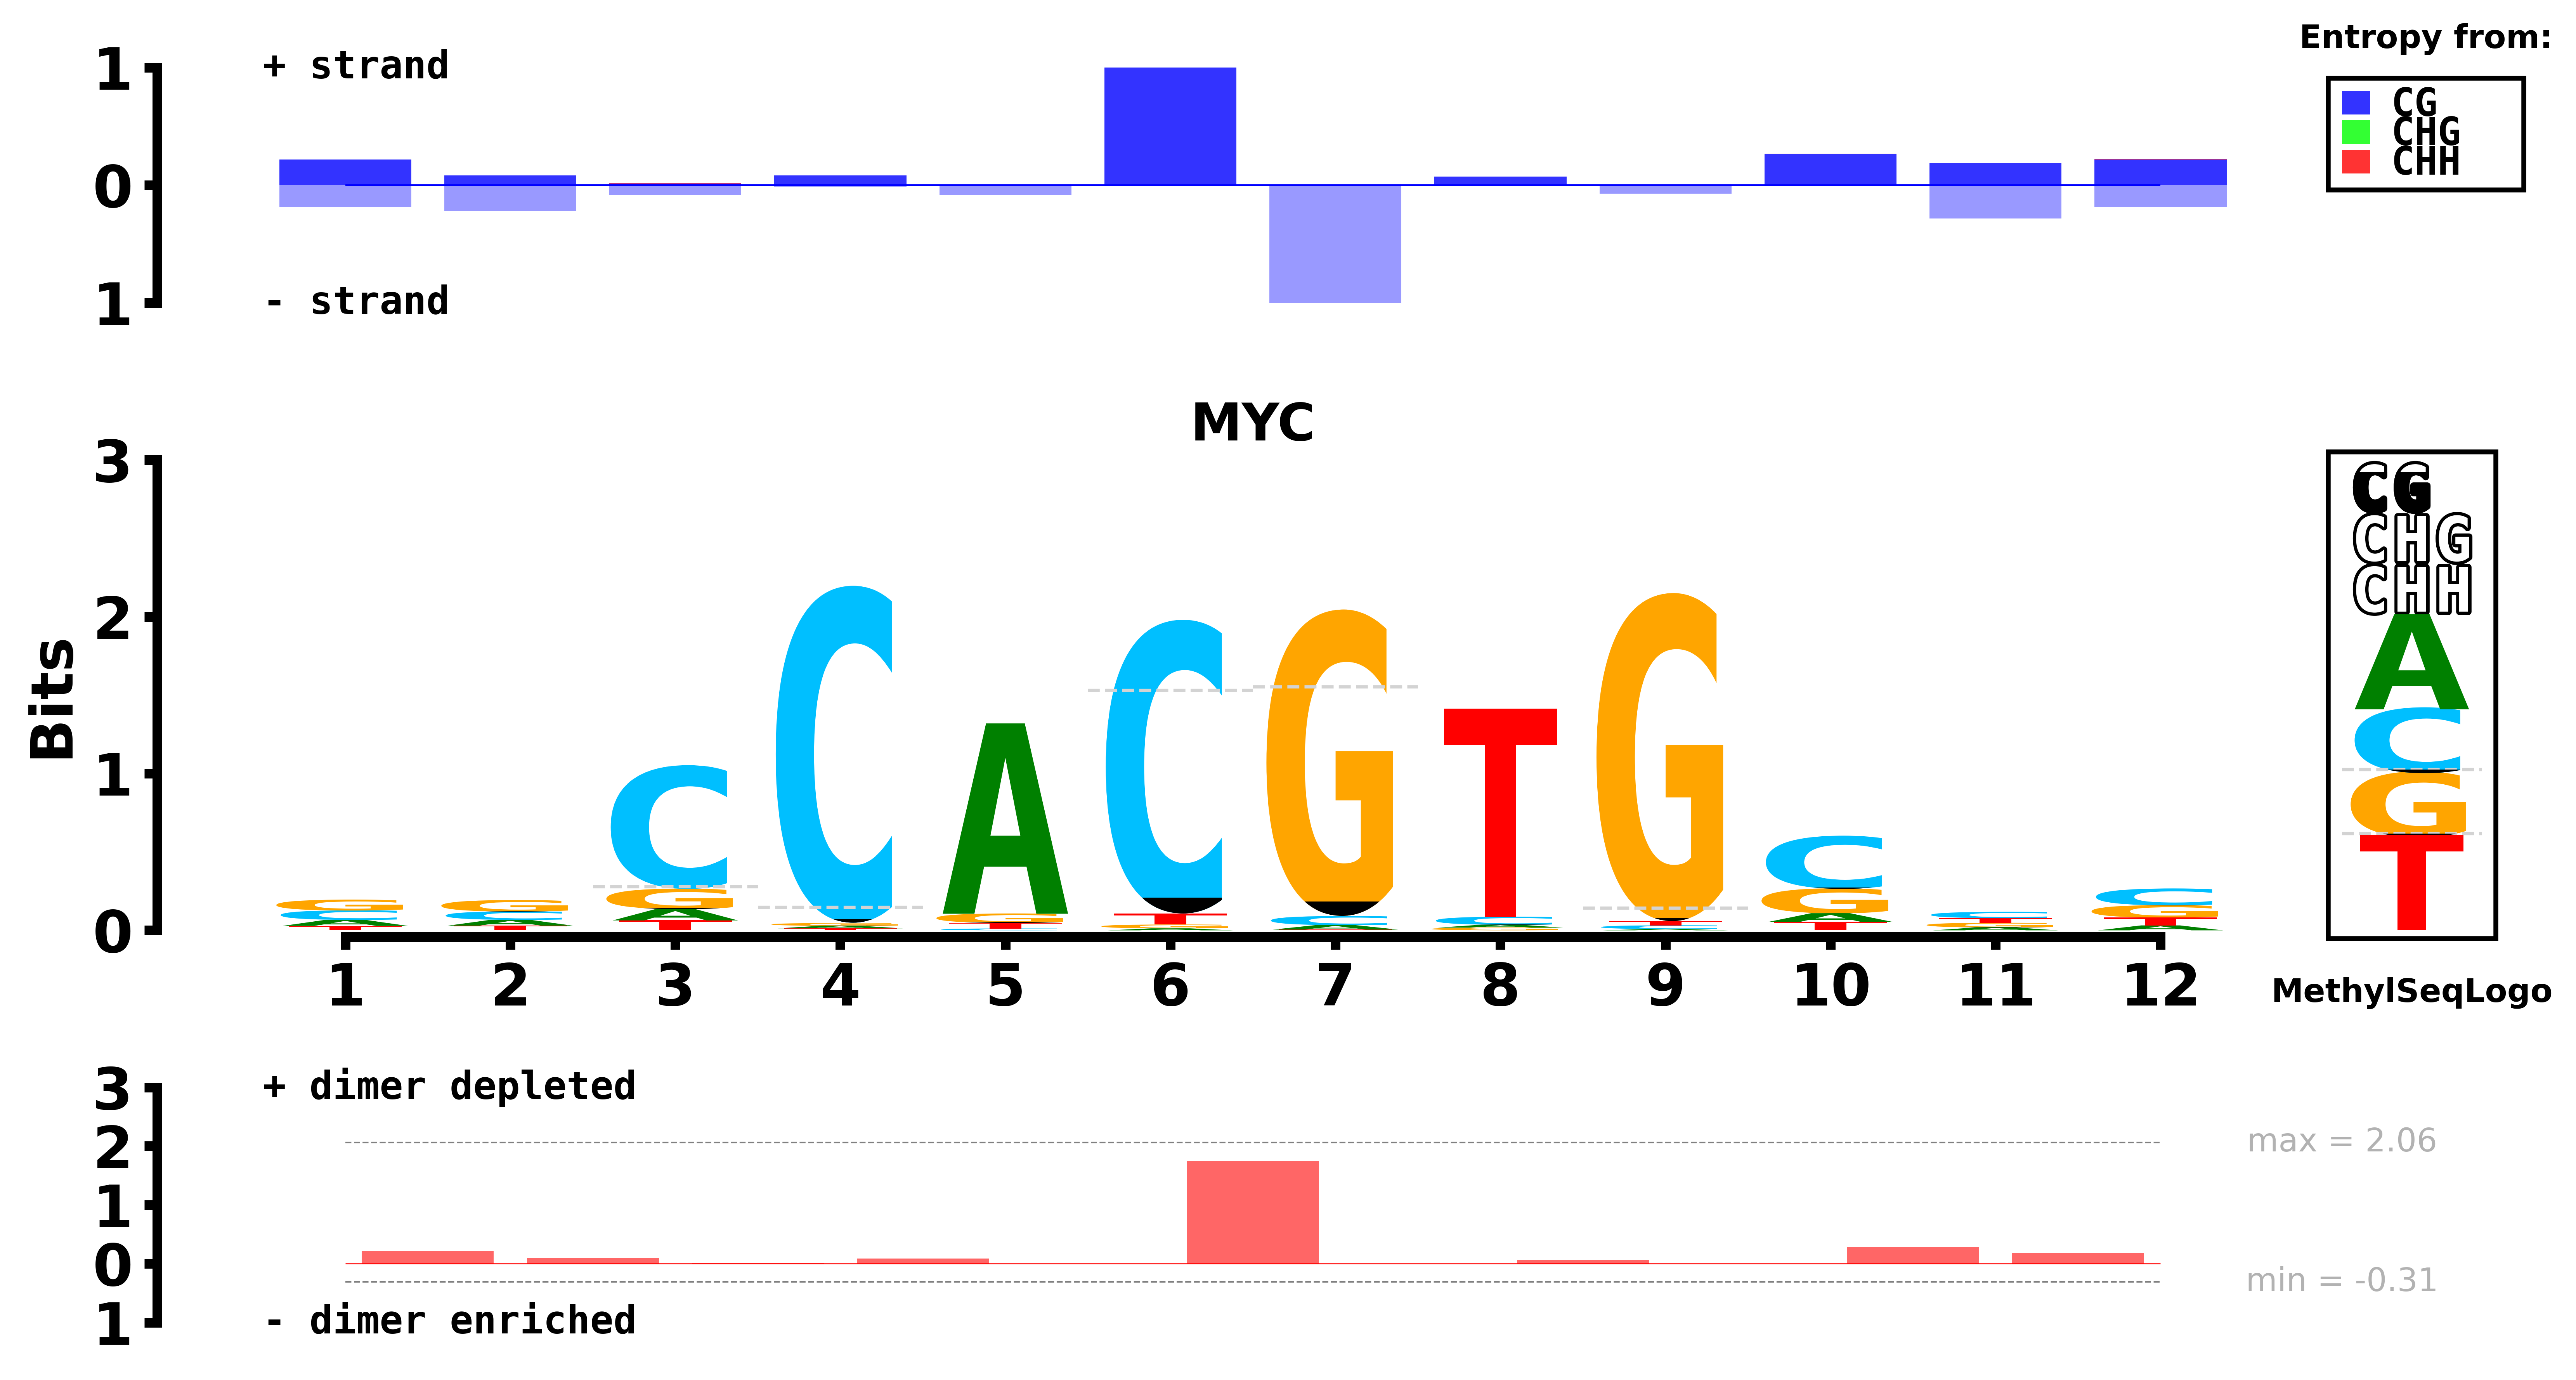
\includegraphics[scale=0.4]{figures/yulingMYC.png}
	\caption{Seqlogo of MYC in H1-hESC cell in whole-genome background model with Kullback-Liebler}
	\label{fig:MYC} 
\end{figure}

\section{CEBPB in H1-hESC cell line}
CEBPB is a transcription factor belonging to the C/EBP (CCAAT/enhancer-binding protein) family. It is widely expressed in mammalian cells, particularly at higher levels in tissues such as the liver, spleen, kidney, and bone marrow. The CEBPB protein contains a basic region that enables it to bind to specific DNA sequences. Additionally, the CEBPB transcription factor includes a leucine zipper structure following the basic region, which is a helix-loop-helix motif facilitating protein-protein interactions to form dimers or multimeric complexes.CEBPB is involved in regulating the production of inflammatory factors, playing a crucial role in immune response and inflammation processes. Furthermore, CEBPB is closely associated with cell proliferation and differentiation, regulating the expression of specific genes in various cell types, thus influencing cell differentiation status and function. In adipocytes, CEBPB is considered one of the key transcription factors involved in adipocyte differentiation. In the study conducted by Ximei Luo et al., they mentioned that CEBPB binding sites were located in highly methylated regions in H1-hESC cell~\cite{luo2021effects}. The dotted lines represent the degree of background methylation, while the black shading indicates the level of methylation at the binding sites. In Figure~\ref{fig:CEBPBFlanking}, the methylation condition of CG at positions 6 and 7 in the motif is prominently displayed, with a substantial area of black shading exceeding the dotted line. The visual representation of the data in the figure aligns with the findings of the study.
\begin{figure}[H]
	\centering
	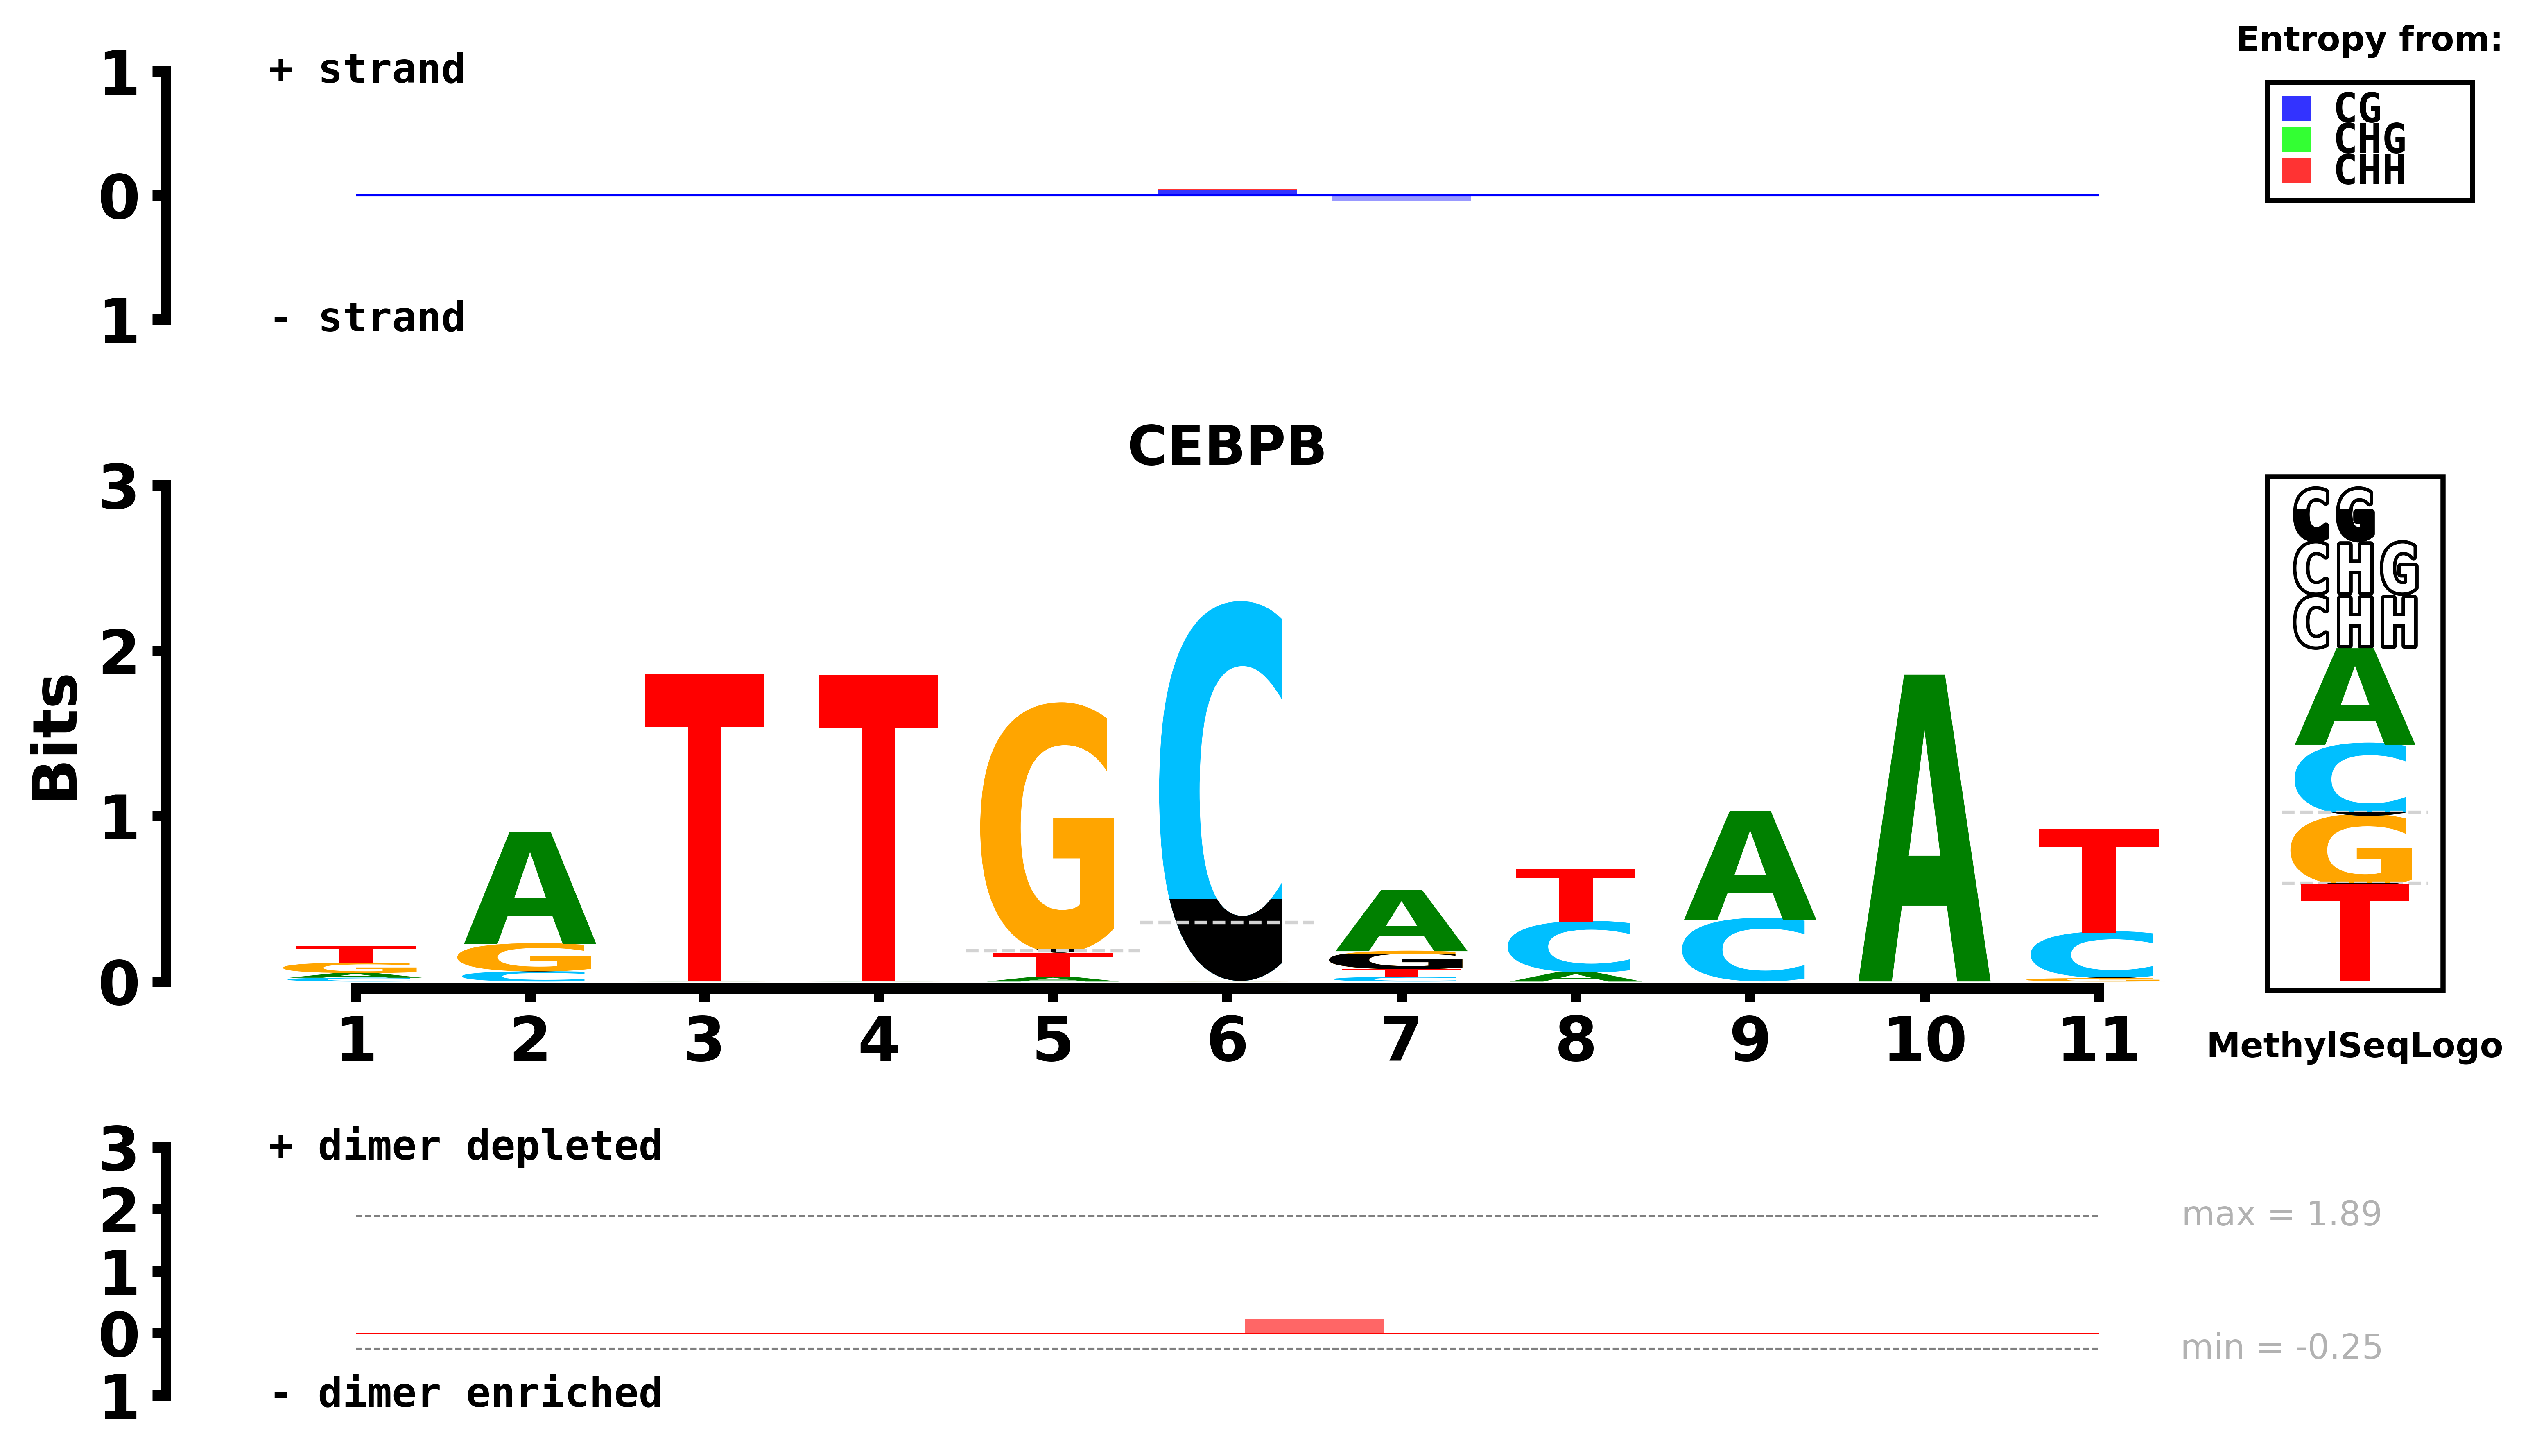
\includegraphics[scale=0.55]{figures/yulingCEBPB_human_H1-hESC_50_Methyl_Kullback-Liebler_seqlogo.png}
	\caption{Seqlogo of CEBPB in H1-hESC cell in flanking region background model with Kullback-Liebler}
	\label{fig:CEBPBFlanking} 
\end{figure}

\chapter{Discussion \& Future Work}
\section{Discussion}
\subsection{JASPAR version affects Sequence Logo Track of MethylSeqLogo}
In this study, the input data utilized a BED file containing specific binding site coordinates of transcription factors in all cells or tissues, which was curated by JASPAR. For each included transcription factor, JASPAR always provides a position weight matrix (PWM) but may not necessarily offer a corresponding BED file. Additionally, there may be multiple versions of the data (as detailed in section 2.3.1), so special attention is required. In the case of the CEBPB transcription factor, this study encountered different versions of the data. The current version available is the 3rd version, which only provides a PWM matrix. The BED file, on the other hand, is only available in version 1. However, the data in versions 1 and 3 differ significantly(shown in Figure~\ref{fig:CEBPBv1v3}), leading to different results in the sequence logo analysis. In a research report, it was shown that the preferred binding sites of the CEBPB transcription factor is ATTGCGCAAT~\cite{johnson1993identification}. Figure~\ref{fig:CEBPBFlanking} presents the results obtained using version 1 (Figure~\ref{fig:CEBPBv1}) of the BED file. The common bases at positions 7 and 8 in motifs on the figure differ from the research findings of~\cite{johnson1993identification}. At first glance, this might lead us to believe that there is an error in the computational pipeline established in this study. However, upon observing the Sequence logo provided by JASPAR in version 3, it becomes evident that the disparities arise from differences in the content of the JASPAR versions. Details like these are worth paying close attention to.
\
\begin{figure}[htbp]
	\centering
	\begin{subfigure}[b]{0.45\textwidth}
		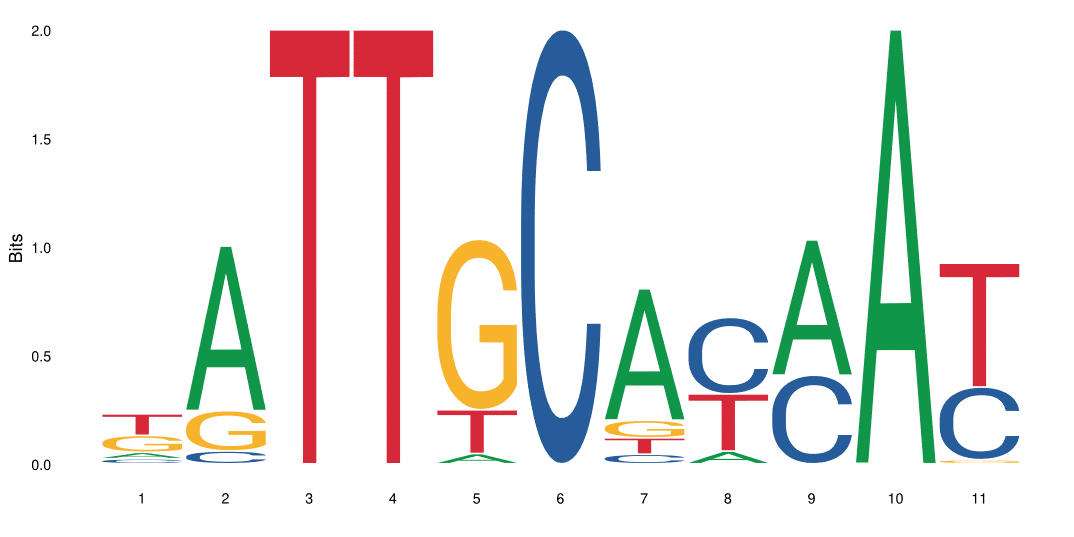
\includegraphics[width=\textwidth]{figures/v1.png}
		\caption{Version 1}
		\label{fig:CEBPBv1} 
	\end{subfigure}
	\begin{subfigure}[b]{0.45\textwidth}
		\ContinuedFloat
		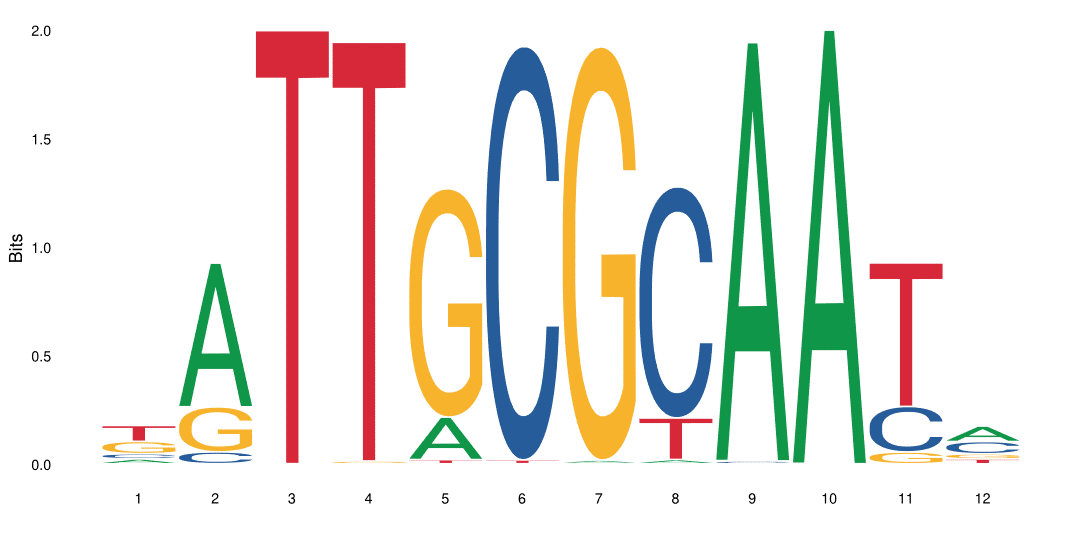
\includegraphics[width=\textwidth]{figures/v3.png}
		\caption{Version 3}
	\end{subfigure}
	\caption{Sequence logo of different versions of CEBPB in JASPAR (without no change)}
	\label{fig:CEBPBv1v3} 
\end{figure}
\subsection{Compare 3 Background Models}
In Figure~\ref{fig:CEBPBFlanking}, we utilized the flanking region background model to illustrate the high methylation status of CEBPB transcription factor binding sites in human embryonic stem cells. However, we have now transitioned to employing the whole genome and promoter region as the background model for statistical distribution calculations. The results, as depicted in Figure~\ref{fig:CEBPBWhole-genome} and Figure~\ref{fig:CEBPBpromotor}, demonstrate that under both the whole genome background model and the flanking region background model, there is a tendency towards high methylation status. Interestingly, the promoter region background model reveals a low methylation pattern, possibly indicating that the majority of CEBPB binding sites are not located within the promoter region. Therefore, the selection of an appropriate background model is crucial depending on the objective of our investigation. In the case of examining the high methylation status of CEBPB binding sites in human embryonic stem cells, the flanking region model and the whole genome model are suitable choices.
\begin{figure}[H]
	\centering
	\begin{subfigure}[b]{0.9\textwidth}
		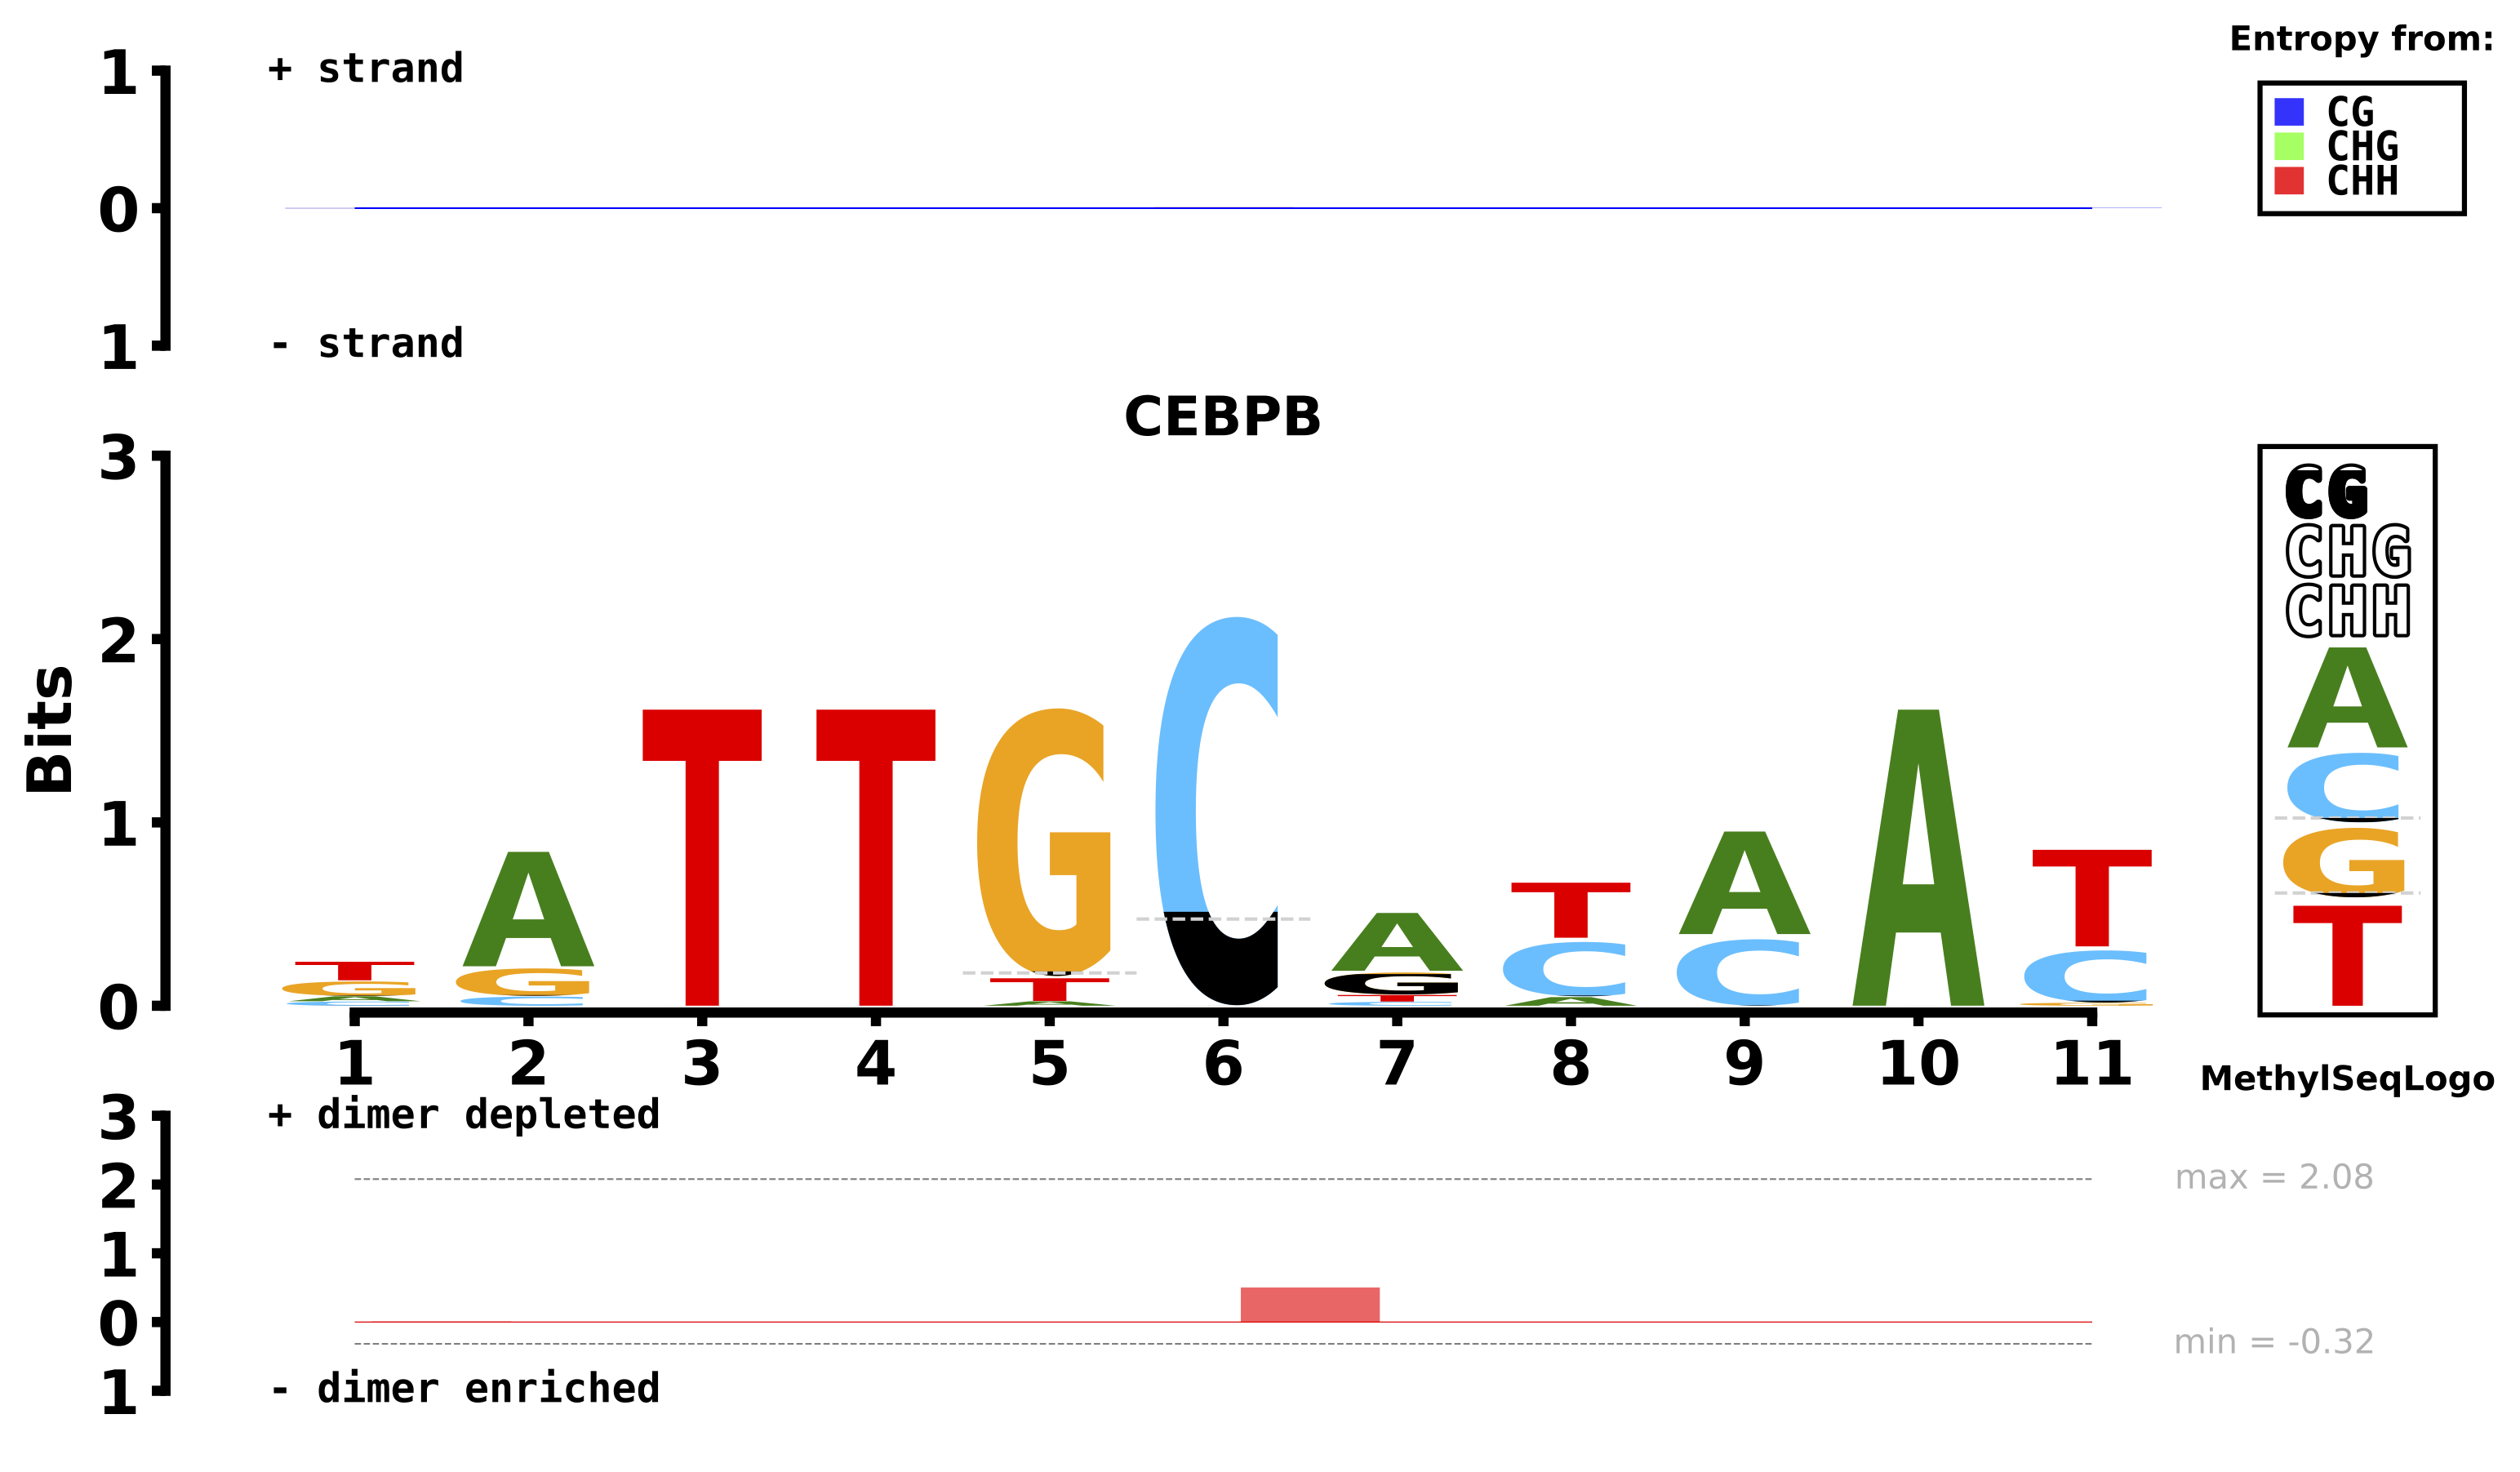
\includegraphics[width=\textwidth]{figures/CEBPBPwg.png}
		\caption{Whole genome}
		\label{fig:CEBPBWhole-genome} 
	\end{subfigure}
	\begin{subfigure}[b]{0.9\textwidth}
		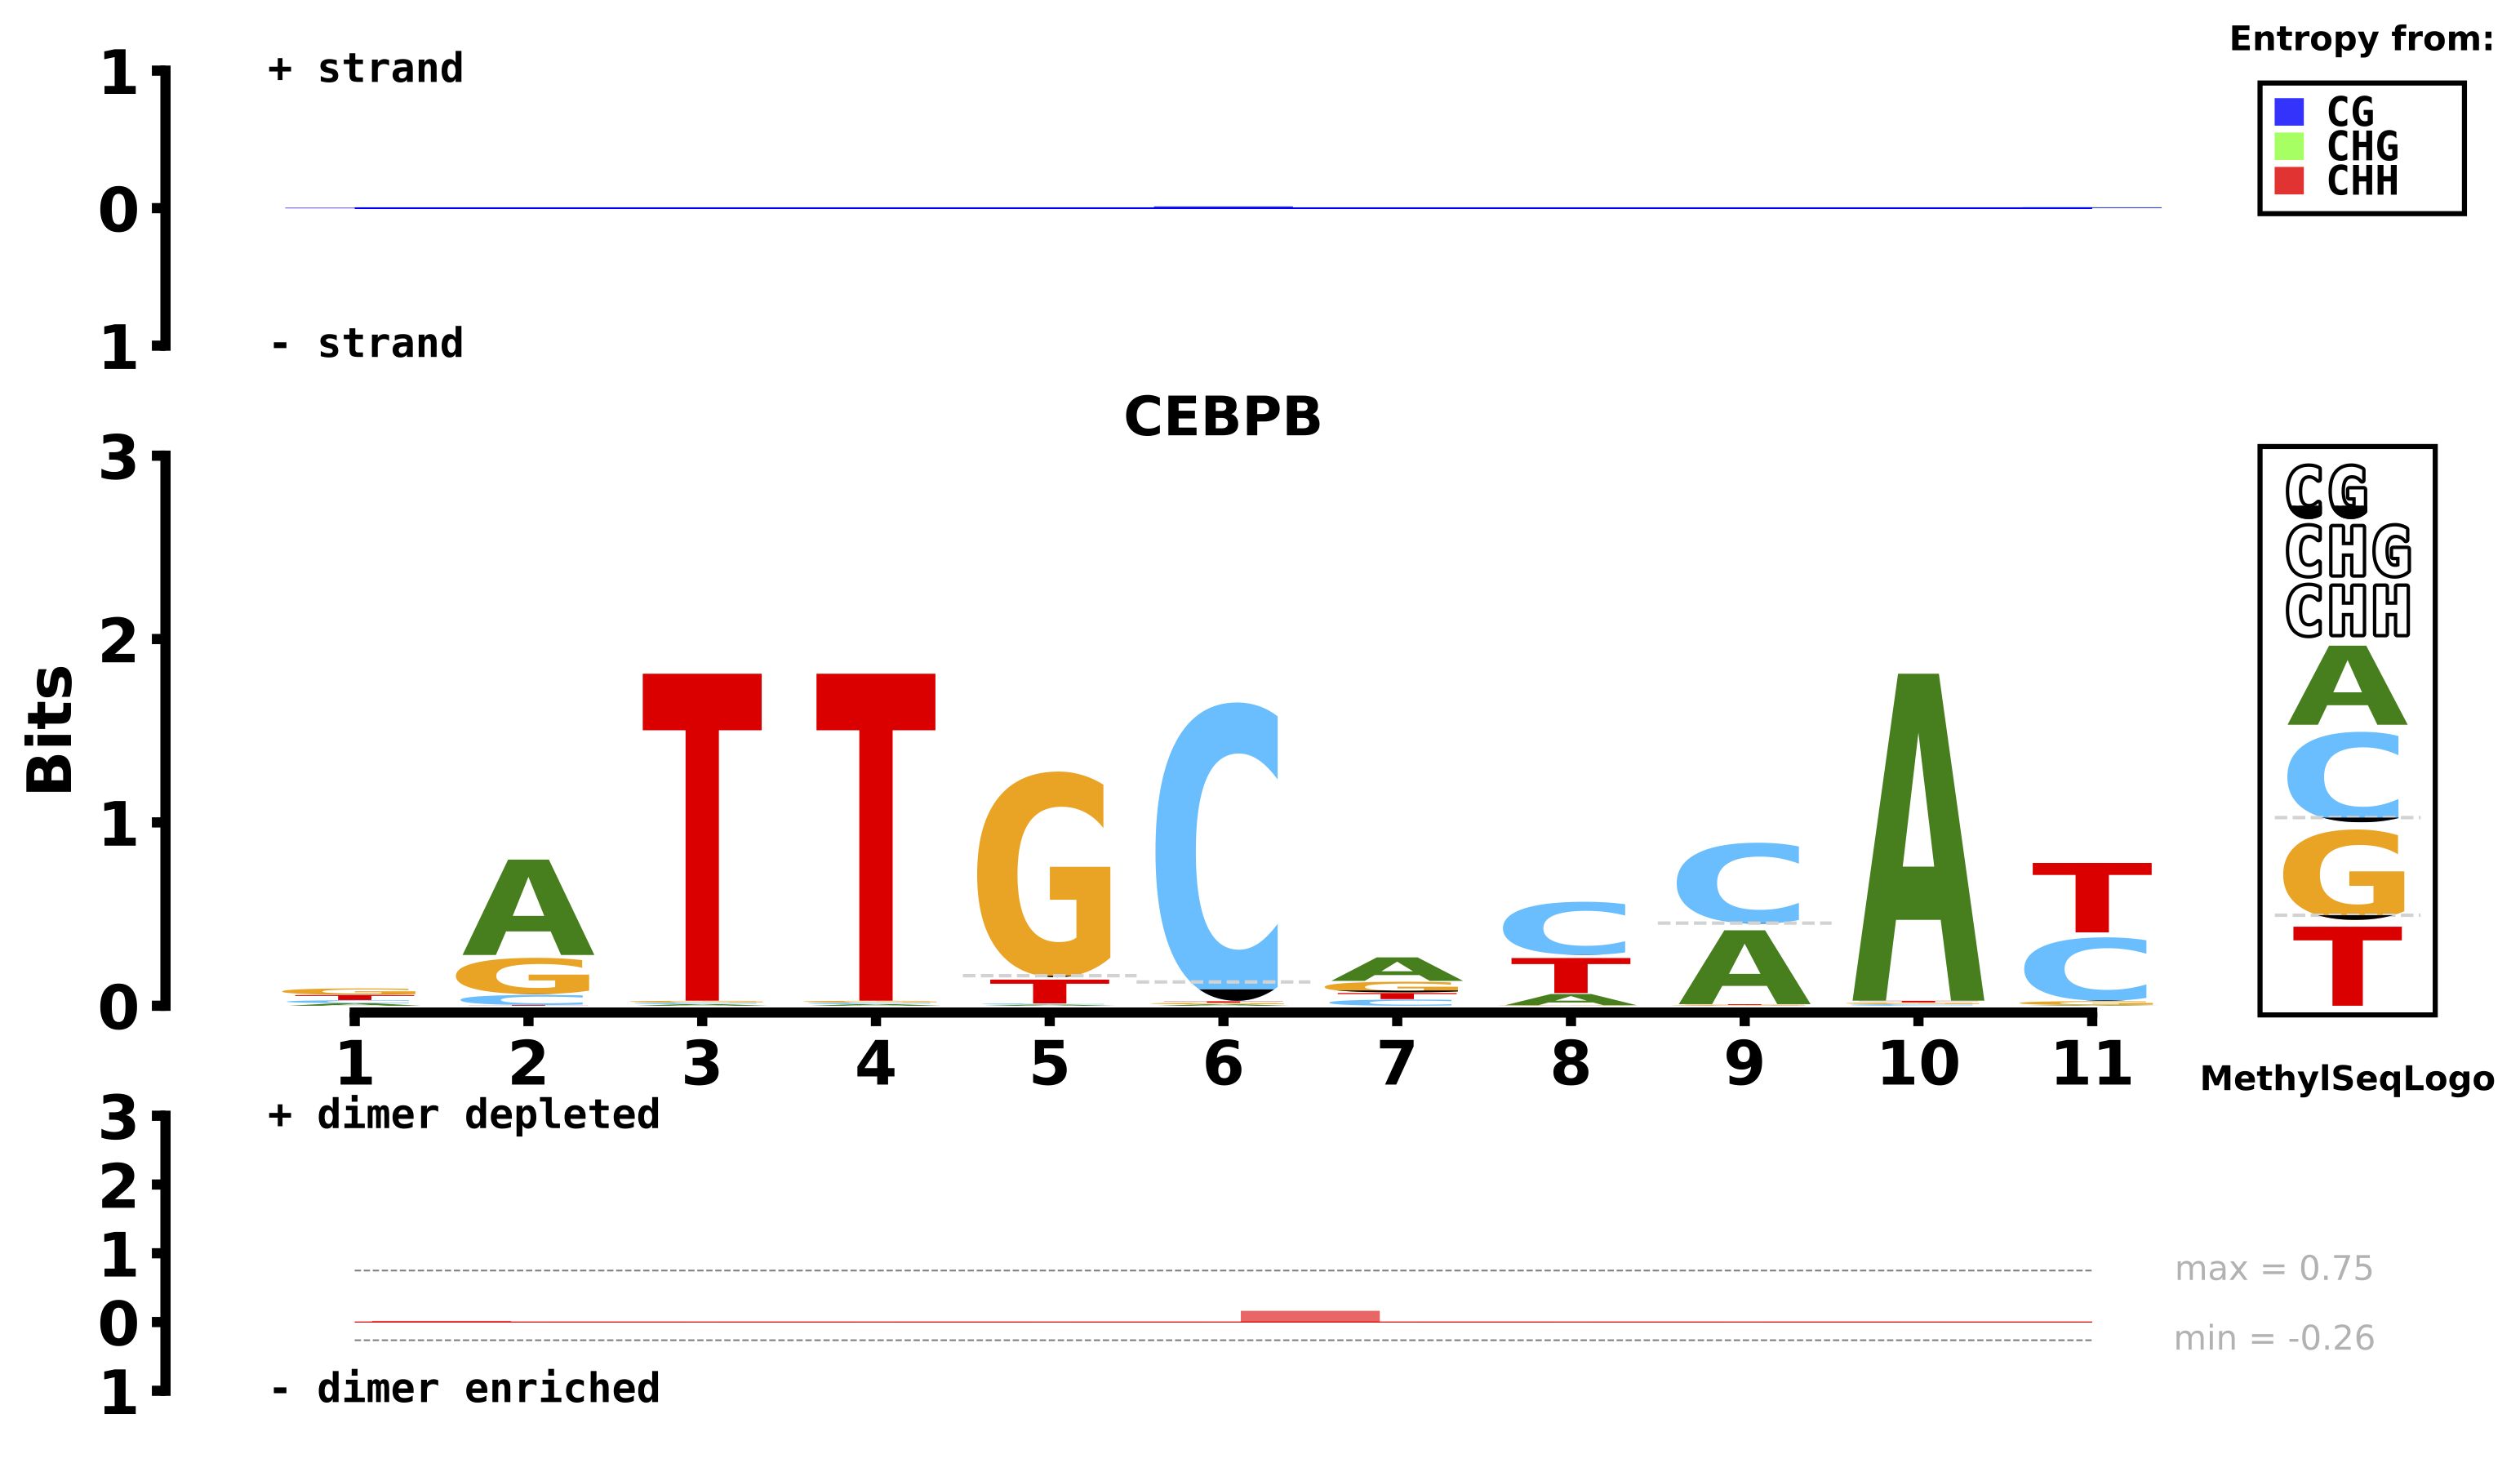
\includegraphics[width=\textwidth]{figures/CEBPBPROMOTOR.png}
		\caption{Promoter region}
		\label{fig:CEBPBpromotor} 
	\end{subfigure}
\end{figure}
	
\begin{figure}[H]
	\ContinuedFloat
	\begin{subfigure}[T]{0.9\textwidth}
		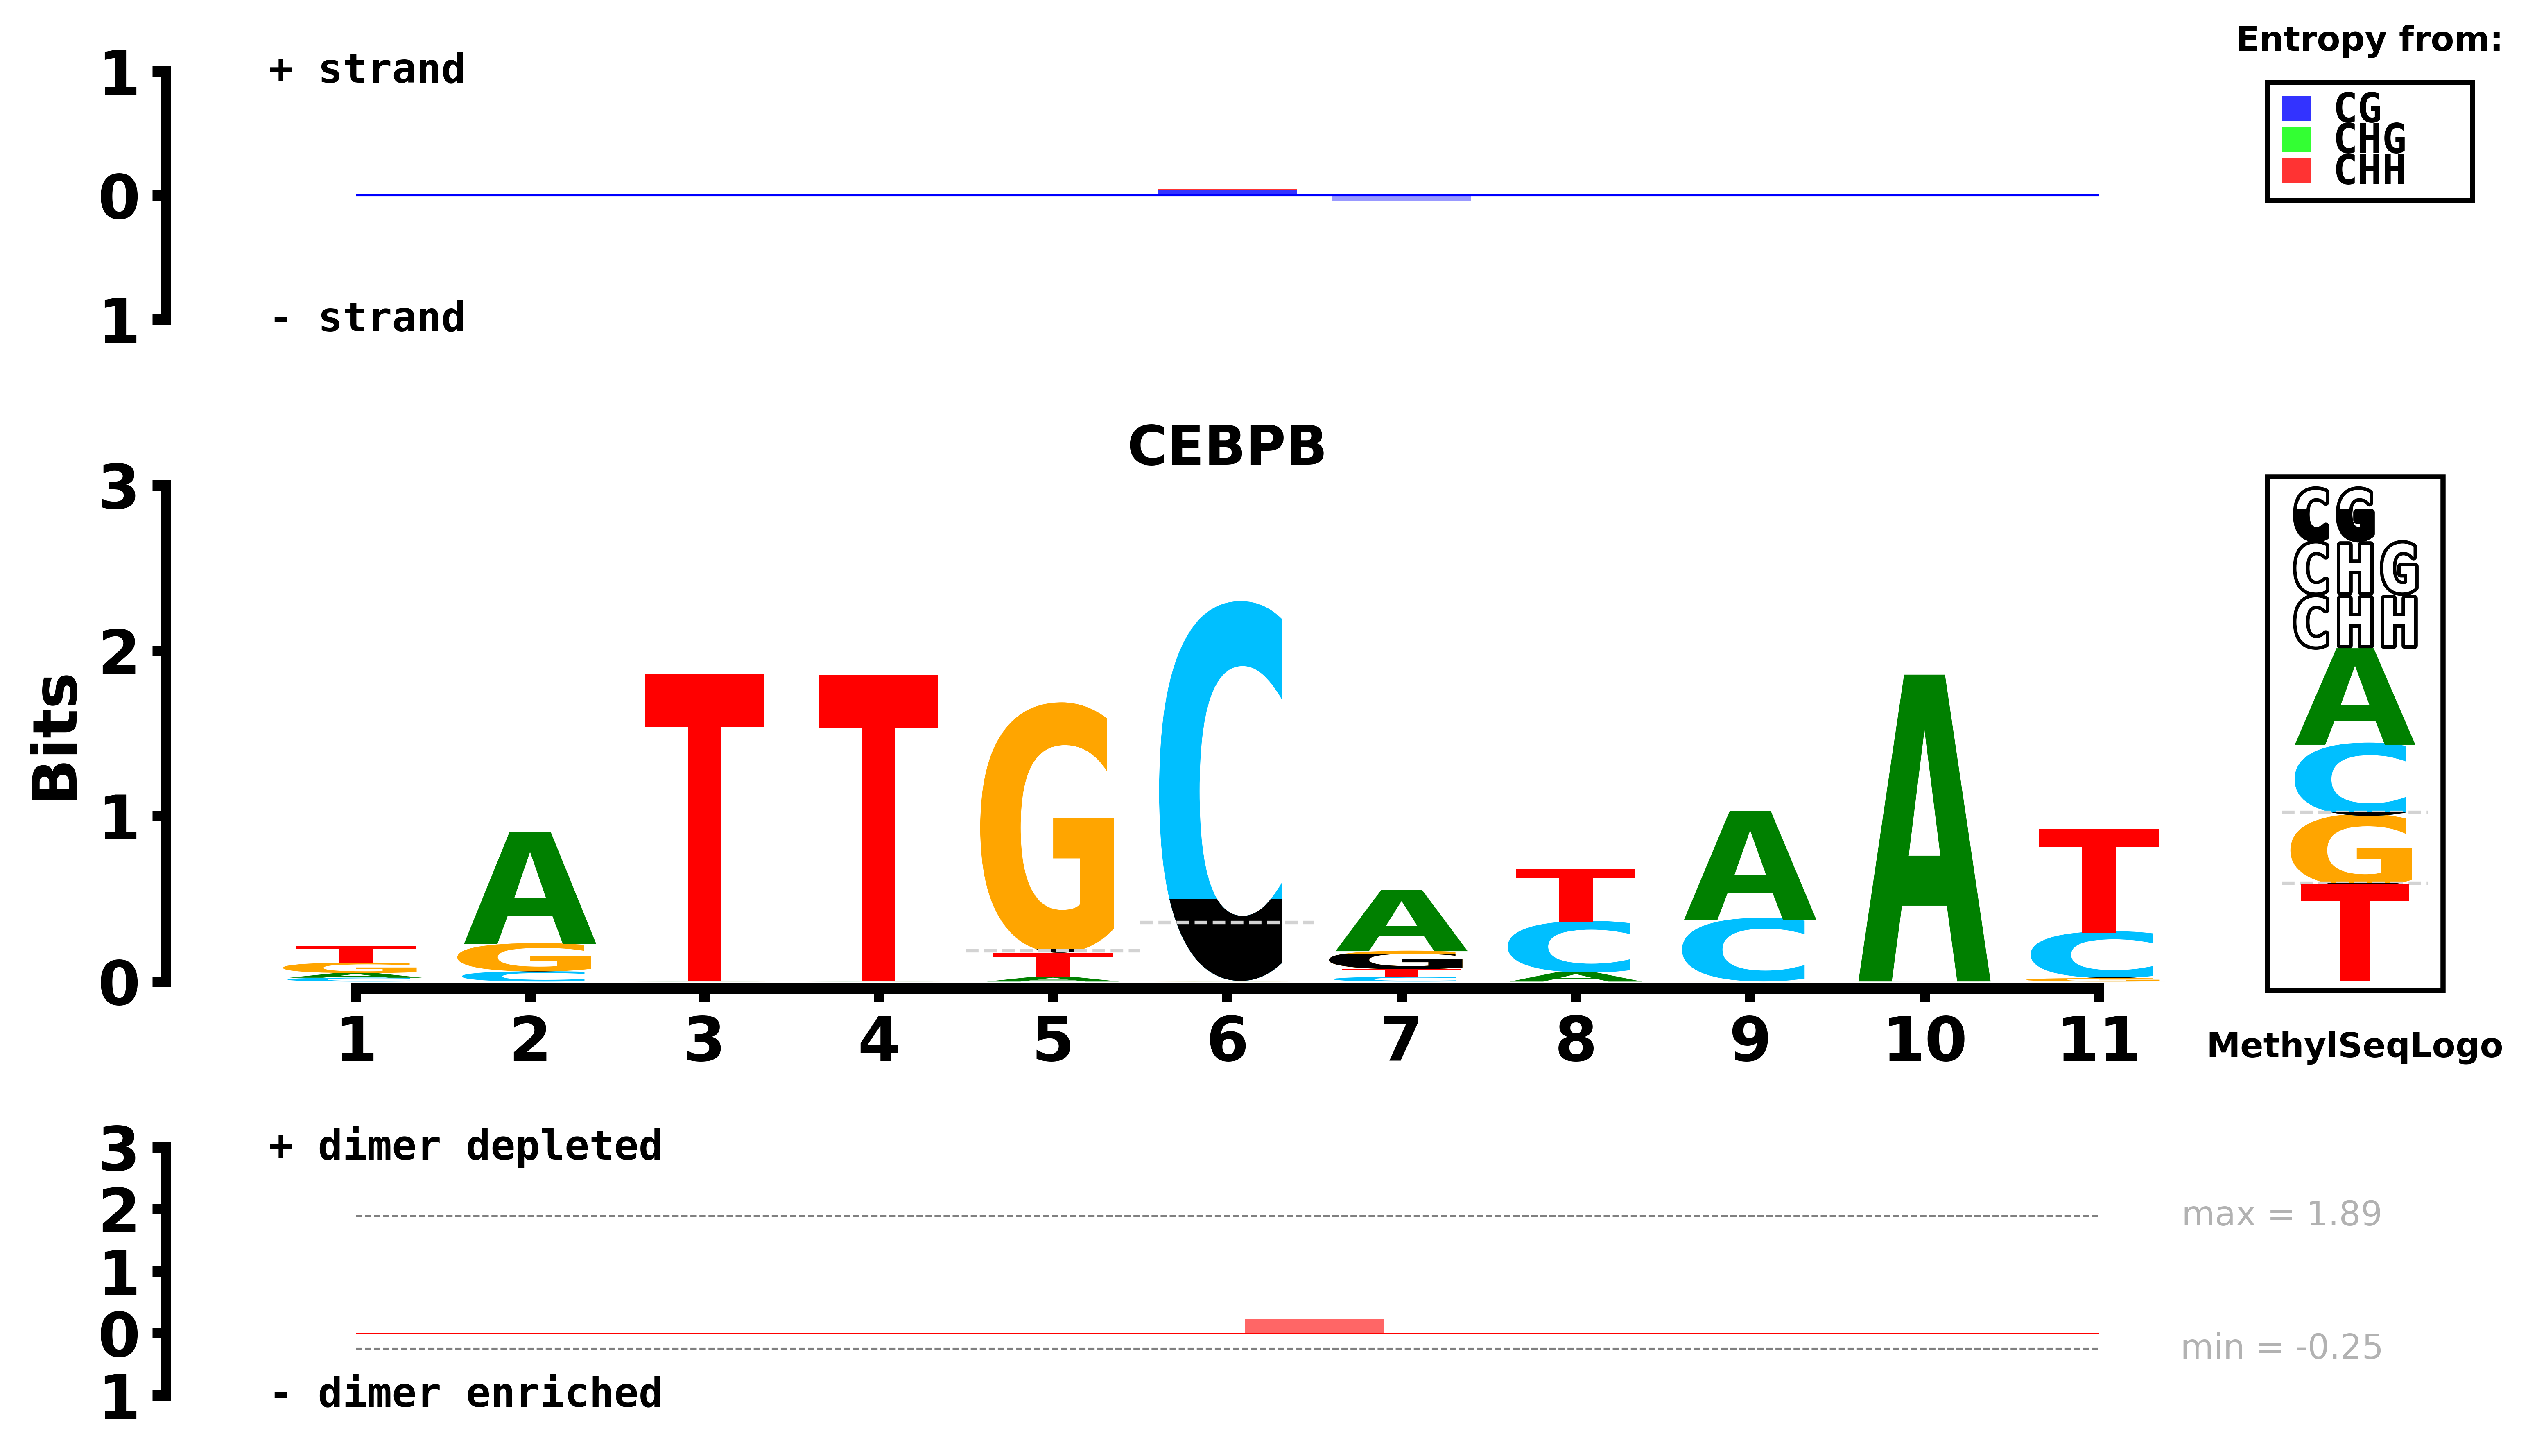
\includegraphics[width=\textwidth]{figures/yulingCEBPB_human_H1-hESC_50_Methyl_Kullback-Liebler_seqlogo.png}
		\caption{Flanking region}
		\label{fig:CEBPBFlanking region} 
	\end{subfigure}
	\caption{MethylSeqLogo of CEBPB TF in H1-hESC cell with different background models}
	\label{fig:CEBPBregion} 
\end{figure}
\subsection{More efficient}
Lastly, I would like to discuss the establishment of an automated computational pipeline in this study. The design of automation not only brings convenience but, more importantly, allows for the rapid generation of results. Before the implementation of the automated computational pipeline, it was estimated that it would take approximately 3 - 4 hours to obtain a single MethylSeqLogo depicting the binding of MYC to human embryonic stem cells using the whole-genome background model. However, with the implementation of the automated computational pipeline, this study can now generate approximately 10 MethylSeqLogos depicting the binding of various transcription factors to human embryonic stem cells in the whole genome background model within the same timeframe.

\section{Future Work}

The accuracy of the input data is a crucial factor influencing MethylSeqLogo. To ensure accurate and reliable visualization, it is important to obtain the latest version of the BED file from JASPAR or similar curated datasets containing transcription factor binding site coordinates. By utilizing the automated pipeline developed in this study, more comprehensive and accurate visual representations can be generated. Additionally, since DNA methylation does not have a direct causal relationship with transcription factor binding, factors such as chromatin structure, signaling pathways, and the environment can also influence transcription factor binding.Furthermore, in the future, it is possible to incorporate additional information onto the sequence logo, such as the information on 5-hydroxymethyl cytosine and other epigenetic modifications (e.g., histone modifications) as proposed by the author of MethylSeqLogo. This approach would enable a multifaceted understanding of transcription factor functionality. Moreover, methylated cytosines (CHG and CHH contexts) are highly abundant in plants. Therefore, when examining transcription factors in plants, it may be beneficial to include information on CHG and CHH in the third track of the logo.Finally, through the automated pipeline software I have developed, users now have the freedom to explore the binding patterns between any transcription factor and cells. However, the usability of the software may be hindered by inconveniences caused by variations in computer environments and devices. In the future, transforming the software into a web-based application would undoubtedly provide users with a more seamless and user-friendly experience in obtaining MethylSeqLogo. By doing so, users would no longer need to navigate obstacles related to their computer equipment, allowing for easier and more accessible access to MethylSeqLogo results.
\chapter{Conclusion}
In this paper, we establish an automated computational pipeline for MethylSeqLogo, which not only provides convenience but also accelerates the generation of results. While previously only one MethylSeqLogo result could be obtained, this study is now capable of producing 10 MethylSeqLogos within the same timeframe. Additionally, a novel background model option, namely the "flanking region," has been introduced to ensure that statistical differences are attributed to binding sites or, at most, adjacent flanking nucleotides.

The experimental results of this study, as presented in the visualized images, are consistent with findings reported by multiple researchers. In future studies, researchers utilizing the automated computational pipeline established in this study can efficiently observe gene regulation within cells, such as the extent of methylation occurrence and binding site preferences. This can contribute to academic research, related analyses, and discussions, and even aid in disease prevention and treatment.
\newpage
\AddToContents{Bibliography}
\printbibliography


\end{document}
